\documentclass[aspectratio=169,10pt]{beamer}

% -----------------------------------------------------------------------------
% Packages
% -----------------------------------------------------------------------------
\usepackage[T1]{fontenc}
\usepackage[utf8]{inputenc}
\usepackage[english]{babel}
\usepackage{lmodern}
\usepackage{amsmath,amssymb,bm}
\usepackage{booktabs}
\usepackage{siunitx}
\usepackage{tikz}
\usepackage{attachfile2}

\usetikzlibrary{arrows.meta,positioning,calc,shapes.geometric,fit,backgrounds}
\usepackage{pgfplots}
\pgfplotsset{compat=1.18}

\usepackage[backend=biber, style=numeric]{biblatex}
\addbibresource{../biblio.bib}

% -----------------------------------------------------------------------------
% Theme
% -----------------------------------------------------------------------------
\definecolor{mainblue}{RGB}{27,74,120}
\definecolor{lightblue}{RGB}{232,240,248}
\definecolor{darkgray}{RGB}{55,60,65}
\definecolor{softgreen}{RGB}{225,242,235}
\definecolor{accentgreen}{RGB}{40,130,90}
\definecolor{softorange}{RGB}{250,238,220}
\definecolor{accentorange}{RGB}{205,120,35}
\definecolor{softred}{RGB}{250,230,230}
\definecolor{accentred}{RGB}{180,60,60}
% Purple colors
\definecolor{accentpurple}{RGB}{125,95,170}
\definecolor{softpurple}{RGB}{242,238,248}

\usetheme{default}
\usefonttheme{professionalfonts}
\setbeamercolor{normal text}{fg=darkgray,bg=white}
\setbeamercolor{frametitle}{fg=mainblue,bg=white}
\setbeamercolor{structure}{fg=mainblue}
\setbeamercolor{alerted text}{fg=accentred}
\setbeamercolor{example text}{fg=accentpurple}
\setbeamertemplate{navigation symbols}{}
\setbeamertemplate{itemize item}{\color{mainblue}$\blacktriangleright$}
\setbeamertemplate{itemize subitem}{\color{mainblue}$\bullet$}
\setbeamertemplate{frametitle}{%
  \vspace{0.15cm}\insertframetitle\par
  \vspace{-0.12cm}\color{mainblue}\rule{\textwidth}{0.5pt}
}
\setbeamertemplate{footline}{%
  \leavevmode%
  \hbox{%
  \begin{beamercolorbox}[wd=.82\paperwidth,ht=2.6ex,dp=1.1ex,leftskip=.35cm]{author in head/foot}%
    \color{gray}\scriptsize Rodolphe Vivant -- Master 2 CSMI -- IRMA / Modartt
  \end{beamercolorbox}%
  \begin{beamercolorbox}[wd=.18\paperwidth,ht=2.6ex,dp=1.1ex,rightskip=.35cm plus1fil]{date in head/foot}%
    \color{gray}\scriptsize \insertframenumber{} / \inserttotalframenumber
  \end{beamercolorbox}}%
}

\setbeamersize{text margin left=0.7cm,text margin right=0.7cm}
\setlength{\abovedisplayskip}{4pt}
\setlength{\belowdisplayskip}{4pt}

% -----------------------------------------------------------------------------
% Helpers
% -----------------------------------------------------------------------------
\newcommand{\keybox}[3][mainblue]{%
  \begin{tikzpicture}[baseline=(n.base)]
    \node[rounded corners=2pt,fill=#1!8,draw=#1!55,inner xsep=7pt,inner ysep=5pt] (n)
    {\begin{minipage}{#2}\centering #3\end{minipage}};
  \end{tikzpicture}%
}
\newcommand{\param}[1]{\ensuremath{#1}}


\newcommand{\bluebox}[2]{%
\begin{tikzpicture}[baseline=(n.base)]
\node[rounded corners=3pt,draw=mainblue!65,fill=lightblue,inner xsep=6pt,inner ysep=5pt] (n)
{\begin{minipage}{#1}\centering #2\end{minipage}};
\end{tikzpicture}}
\newcommand{\orangebox}[2]{%
\begin{tikzpicture}[baseline=(n.base)]
\node[rounded corners=3pt,draw=accentorange!80,fill=softorange,inner xsep=6pt,inner ysep=5pt] (n)
{\begin{minipage}{#1}\centering #2\end{minipage}};
\end{tikzpicture}}
\newcommand{\greenbox}[2]{%
\begin{tikzpicture}[baseline=(n.base)]
\node[rounded corners=3pt,draw=accentgreen!75,fill=softgreen,inner xsep=6pt,inner ysep=5pt] (n)
{\begin{minipage}{#1}\centering #2\end{minipage}};
\end{tikzpicture}}
\newcommand{\purplebox}[2]{%
\begin{tikzpicture}[baseline=(n.base)]
\node[
    rounded corners=3pt,
    draw=accentpurple!75,
    fill=softpurple,
    inner xsep=6pt,
    inner ysep=5pt
] (n)
{\begin{minipage}{#1}\centering #2\end{minipage}};
\end{tikzpicture}}

\title{Automated Calibration of Physical Models\\for Musical Reed Wind Instruments}
\subtitle{Differentiable numerical simulation and inverse calibration}
\author{Rodolphe Vivant}
\institute{Master 2 CSMI -- IRMA, Université de Strasbourg -- Modartt}
\date{Master's thesis defense -- August 27, 2026}

\begin{document}

% =============================================================================
% 1. TITLE
% =============================================================================
\begin{frame}[plain]

\vspace{0.35cm}

% -------------------------------------------------------------------------
% TITLE
% -------------------------------------------------------------------------
\begin{center}

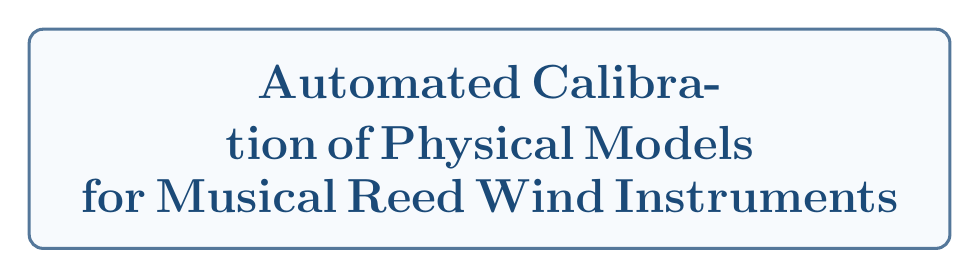
\begin{tikzpicture}
\node[
    rounded corners=5pt,
    draw=mainblue!75,
    line width=1.1pt,
    fill=lightblue!35,
    inner xsep=18pt,
    inner ysep=13pt,
    text width=0.86\linewidth,
    align=center
] {
    {\LARGE\bfseries\color{mainblue}
    Automated Calibration of Physical Models\\[0.10cm]
    for Musical Reed Wind Instruments}
};
\end{tikzpicture}

\vspace{0.60cm}

{\LARGE\bfseries
Rodolphe Vivant
\par}

\vspace{0.15cm}

{\normalsize
Master 2 CSMI -- Université de Strasbourg
\par}

\vspace{0.10cm}

{\small
August 27, 2026
\par}

\end{center}


% -------------------------------------------------------------------------
% SUPERVISION
% -------------------------------------------------------------------------
\vspace{0.25cm}

\begin{columns}[T,onlytextwidth]

\column{0.48\textwidth}
\centering
\small

\textbf{\color{mainblue}Academic supervisors}

\vspace{0.12cm}

Emmanuel Franck\\
Laurent Navoret\\
Victor Michel-Dansac


\column{0.48\textwidth}
\centering
\small

\textbf{\color{mainblue}Industrial supervisors}

\vspace{0.12cm}

Juliette Chabassier\\
Alexis Thibault

\end{columns}


% -------------------------------------------------------------------------
% LOGOS
% -------------------------------------------------------------------------

\vspace{-0.35cm}
\begin{center}

\begin{minipage}[c]{0.27\linewidth}
    \centering
    
\includegraphics[
        height=0.78cm,
        keepaspectratio
    ]{../Images/logo_irma.png}
\end{minipage}
%
\hspace{-0.02\linewidth}
%
\begin{minipage}[c]{0.27\linewidth}
    \centering
    
\includegraphics[
        height=1.8cm,
        keepaspectratio
    ]{../Images/inria_logo.png}
\end{minipage}
%
\hspace{-0.02\linewidth}
%
\begin{minipage}[c]{0.27\linewidth}
    \centering
    
\includegraphics[
        height=1.8cm,
        keepaspectratio
    ]{../Images/modartt_logo.png}
\end{minipage}

\end{center}

\vspace{0.25cm}

\end{frame}

% =============================================================================
% 2. CONTEXT AND OBJECTIVES
% =============================================================================
\begin{frame}{Context \& Objectives}
    \vspace{-0.15cm}
\begin{columns}[T,onlytextwidth]
\column{0.52\textwidth}
\small
\textbf{Goal of the internship}
\vspace{-0.1cm}
\begin{itemize}
  \item Automatically calibrate a physical model of reed wind instruments from acoustic observations.
  \item Joint collaboration between IRMA (Université de Strasbourg) and Modartt \footnotemark[1] (Modartt SAS, Paris).
  \item Use differentiable numerical simulation to compute gradients with respect to physical parameters and functionnal.
  \item Assess the method on synthetic OpenWind \footnotemark[2] signals.
\end{itemize}
\vspace{-0.1cm}
\orangebox{0.93\linewidth}{\textbf{Central question}\\[1mm]
Can unknown reed parameters and functional forms be recovered from the sound produced by the instrument?}

\column{0.44\textwidth}
In Jax framework :

\vspace{0.15cm}
\centering
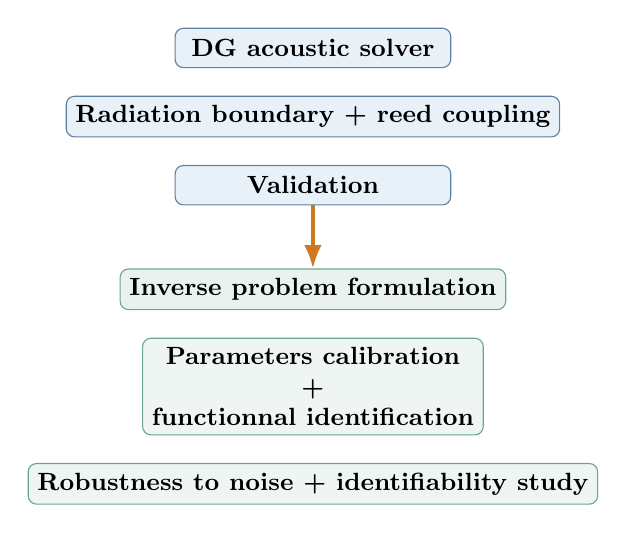
\begin{tikzpicture}[node distance=0.35cm,>=Latex]
\tikzset{b/.style={rounded corners=3pt,draw=mainblue!70,fill=lightblue,minimum width=3.5cm,minimum height=0.5cm,align=center,font=\small\bfseries}}
\node[b] (p1) {DG acoustic solver};
\node[b,below=of p1] (p2) {Radiation boundary + reed coupling};
\node[b,below=of p2] (p3) {Validation};
\node[b,below=0.8cm of p3,fill=accentgreen!10,draw=accentgreen!70] (s1) {Inverse problem formulation};
\node[b,below=of s1,fill=accentgreen!8,draw=accentgreen!70] (s2) {Parameters calibration \\ + \\ functionnal identification};
\node[b,below=of s2,fill=accentgreen!8,draw=accentgreen!70] (s3) {Robustness to noise + identifiability study};
\draw[->,very thick,accentorange] (p3)--(s1);
\end{tikzpicture}
\end{columns}

\footnotetext[1]{
{\footnotesize \cite{Modartt}
\url{https://www.modartt.com/}}
}
\footnotetext[2]{
{\footnotesize \cite{OpenwindInria}
\url{http://openwind.inria.fr}}
}

\end{frame}


\begin{frame}{Reed Wind Instrument Model}
  \begin{center}
        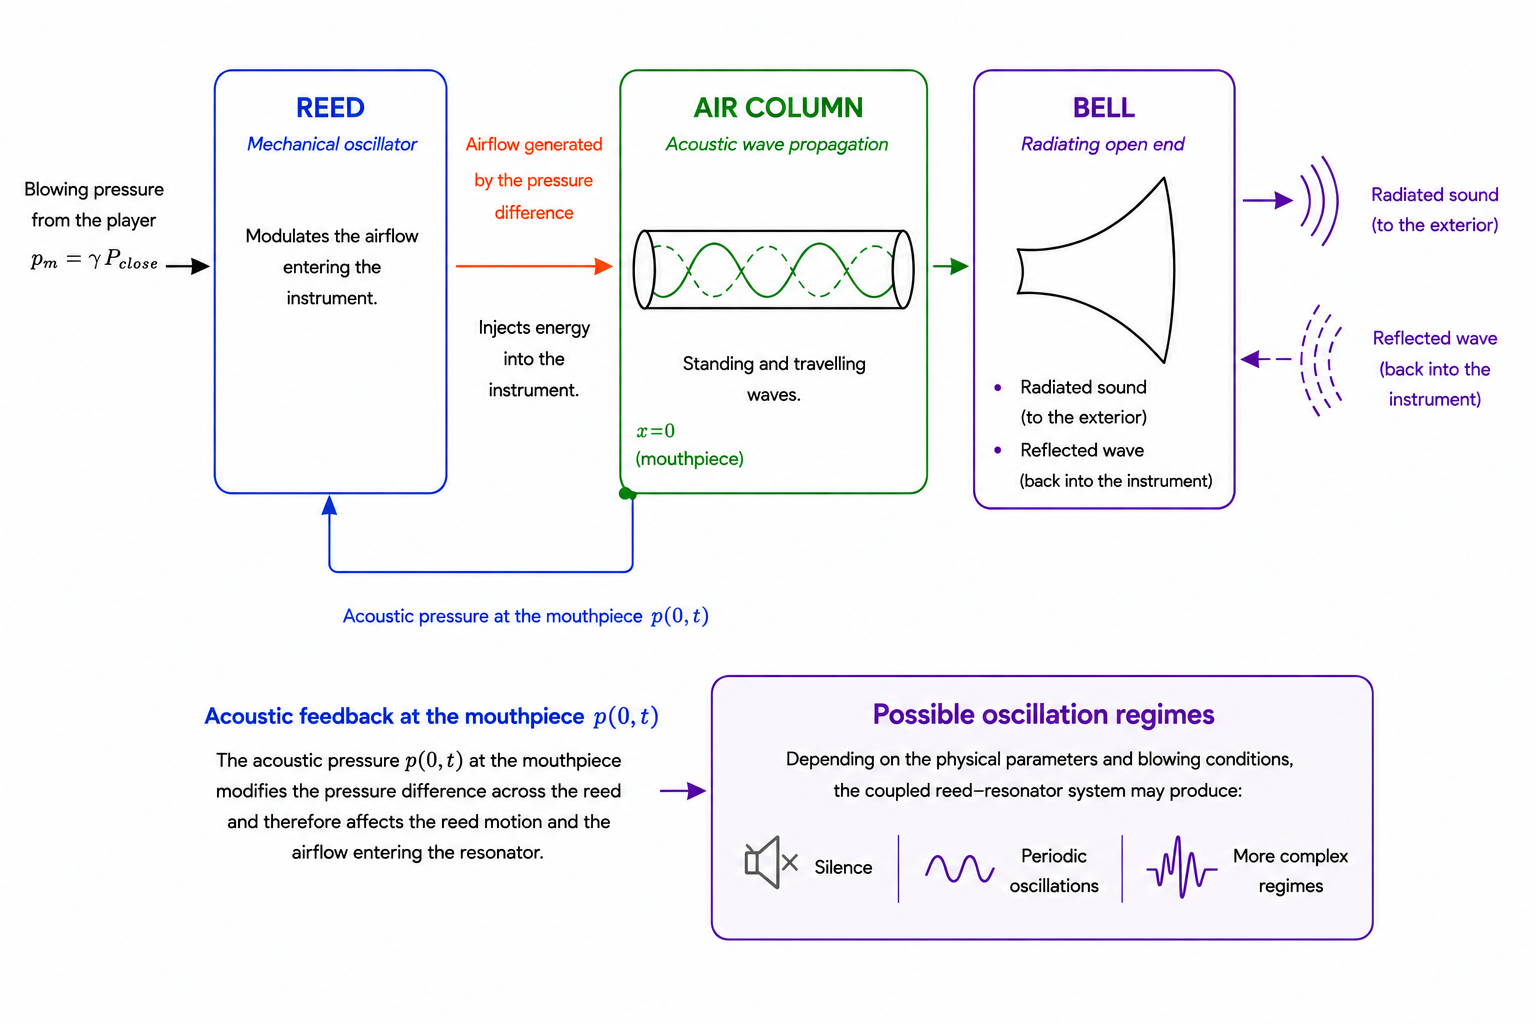
\includegraphics[width=0.6\linewidth,keepaspectratio]{../Images/generation_onde_anche.png}\hspace{0.0em}%
        \par\smallskip
        \scriptsize Illustration of the sound generation mechanism in a single-reed instrument (adapted from \footnotemark[1] \footnotemark[2]).
        \label{fig:generation_onde_anche}  
    \end{center}
\footnotetext[1]{
\footnotesize \cite[Chapter~2]{vergez2010analyse}
Vergez Christophe (2010) \emph{Analyse et modélisation des instruments à vent à anche simple}
}
\footnotetext[2]{
\footnotesize \cite{chaigne:hal-05370840}
Chaigne, Antoine and Kergomard, Jean (2022), \emph{Acoustique des instruments de musique}
}
\end{frame}

  % =============================================================================
  % 3. PHYSICAL MODEL
  % =============================================================================
  \begin{frame}{Physical Model}
    \vspace{-0.25cm}
  \begin{columns}[T,onlytextwidth]
  \column{0.57\textwidth}
  \small
  \textbf{Acoustic propagation in a variable-section resonator} \footnotemark[1]\footnotemark[2]
  \vspace{-0.25cm}
  \begin{align*}
  \frac{S(x)}{cS^*}\partial_t p + \partial_x v &=0, &
  \frac{S^*}{cS(x)}\partial_t v + \partial_x p &=0.
  \end{align*}

  \vspace{-0.25cm}
  \textbf{Reed oscillator}
  \vspace{-0.15cm}
  \[
  \frac{1}{\omega_r^2}\partial_{tt}y+
  \frac{1}{Q_r\omega_r}\partial_ty+y-1
  =\varepsilon\bigl(\gamma-p(0,t)\bigr).
  \]

  \vspace{-0.25cm}
  \textbf{Nonlinear mouthpiece coupling}
  \vspace{-0.25cm}
  \[
  -v(0,t)+\zeta\ell(y)F\bigl(\gamma-p(0,t)\bigr)
  +\varepsilon\frac{\kappa}{\omega_r}\partial_ty=0.
  \]
  \vspace{-0.55cm}
  \[
  F(\Delta p)=\operatorname{sign}(\Delta p)\sqrt{|\Delta p|}.
  \]

  \vspace{-0.15cm}
  \textbf{Radiative boundary condition}
  \vspace{-0.25cm}
  \[ 
  Z^\ast_T\,\partial_t \phi + \sqrt{\alpha}\,p(L,t) = 0
  \]
  \vspace{-0.65cm}
  \[
  -\frac{\beta}{Z^\ast_T}\,p(L,t) + v(L,t) + \sqrt{\alpha}\,\phi = 0
  \]
    \vspace{-0.5cm}
  with \[
    p,v:(0,L)\times(0,T)\rightarrow\mathbb R,
    \qquad
    y,\phi:(0,T)\rightarrow\mathbb R.
    \]

  \column{0.39\textwidth}
  \centering
  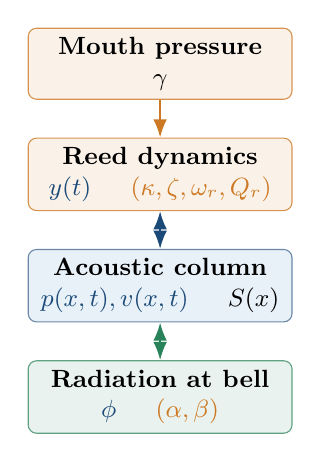
\begin{tikzpicture}[node distance=0.48cm,>=Latex]
  \tikzset{m/.style={rounded corners=3pt,draw=mainblue!65,fill=lightblue,minimum width=3.35cm,minimum height=0.85cm,align=center,font=\small\bfseries}}
  \tikzset{mainblue/.append style={color=mainblue}}
  \tikzset{accentorange/.append style={color=accentorange}}
  \tikzset{accentgreen/.append style={color=accentgreen}}
  \node[m,fill=accentorange!10,draw=accentorange!80] (mouth) {Mouth pressure\\$\gamma$};
  \node[m,below=of mouth,fill=accentorange!10,draw=accentorange!80] (reed) {Reed dynamics\\
$\textcolor{mainblue}{y(t)}$
\quad
$\textcolor{accentorange}{(\kappa,\zeta,\omega_r,Q_r)}$};
  \node[m,below=of reed] (tube) {Acoustic column\\
$\textcolor{mainblue}{p(x,t),v(x,t)}$
\quad
$S(x)$};
  \node[m,below=of tube,fill=accentgreen!10,draw=accentgreen!75] (bell) {Radiation at bell\\$\textcolor{mainblue}{\phi}$ \quad $\textcolor{accentorange}{(\alpha,\beta)}$};
  \draw[->,thick,accentorange] (mouth)--(reed);
  \draw[<->,thick,mainblue] (reed)--(tube);
  \draw[<->,thick,accentgreen] (tube)--(bell);
  \end{tikzpicture}
  \vspace{0.1cm}

  \bluebox{0.92\linewidth}{\small PDE + ODE + nonlinear boundary conditions}
  \end{columns}

  \footnotetext[1]{
{\footnotesize \cite{thibault}
Thibault, Alexis (2023), \emph{Mod{\'e}lisation, analyse et simulation de l'acoustique dissipative dans les tubes poreux ou rugueux : application aux instruments {\`a} vent}}
}
  \footnotetext[2]{
{\footnotesize \cite{chabassier:hal-03794382}
Chabassier, Juliette and Auvray, Roman (2022), Control Parameters for Reed Wind Instruments or Organ Pipes with Reed Induced Flow}
}
\end{frame}

% =============================================================================
% INVERSE PROBLEM — MOTIVATION
% =============================================================================
\begin{frame}{From Sound to Model Parameters}

\vspace{-0.25cm}

\begin{columns}[T,onlytextwidth]

% -------------------------------------------------------------------------
% LEFT : TARGET SOUND
% -------------------------------------------------------------------------
\column{0.29\textwidth}

\centering

\textbf{\color{mainblue}Target sound}

\vspace{0.25cm}

\textattachfile[
    mimetype=audio/mpeg,
    description={Experimental trumpet recording},
    color=0 0 1
]{trumpet_sound5_61-63s.mp3}{%
    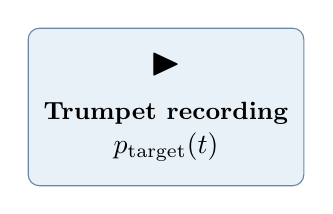
\begin{tikzpicture}
    \node[
        rounded corners=4pt,
        draw=mainblue!65,
        fill=lightblue,
        minimum width=3.5cm,
        minimum height=2.0cm,
        align=center
    ] {
        \Large $\blacktriangleright$\\[0.15cm]
        \small \textbf{Trumpet recording}\\
        $p_{\mathrm{target}}(t)$
    };
    \end{tikzpicture}%
}

\vspace{0.25cm}

{\scriptsize
Sound we would like the model\\
to reproduce.
}


% -------------------------------------------------------------------------
% CENTER : PHYSICAL MODEL
% -------------------------------------------------------------------------
\column{0.39\textwidth}

\centering

\textbf{\color{mainblue}Physical model}

\vspace{0.15cm}

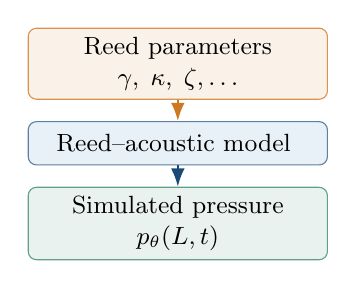
\begin{tikzpicture}[
    node distance=0.27cm,
    >=Latex,
    b/.style={
        rounded corners=3pt,
        minimum width=3.8cm,
        minimum height=0.55cm,
        align=center,
        font=\small
    }
]

\node[
    b,
    draw=accentorange!80,
    fill=accentorange!10
] (reed) {
    Reed parameters\\
    $\gamma,\;\kappa,\;\zeta,\ldots$
};

\node[
    b,
    below=of reed,
    draw=mainblue!70,
    fill=lightblue
] (solver) {
    Reed--acoustic model
};

\node[
    b,
    below=of solver,
    draw=accentgreen!75,
    fill=accentgreen!10
] (output) {
    Simulated pressure\\
    $p_{\theta}(L,t)$
};

\draw[->,thick,accentorange] (reed)--(solver);
\draw[->,thick,mainblue] (solver)--(output);

\end{tikzpicture}

\vspace{0.18cm}

\only<1>{
\orangebox{0.92\linewidth}{
\small
\textbf{How should we choose the parameters}\\
to reproduce the target sound?
}
}

\only<2->{
\greenbox{0.92\linewidth}{
\small
Compare the simulated and target sounds
and adjust the parameters automatically.
}
}


% -------------------------------------------------------------------------
% RIGHT : SIMULATED SOUND
% -------------------------------------------------------------------------
\column{0.29\textwidth}

\centering

\textbf{\color{mainblue}Simulated sound}

\vspace{0.25cm}

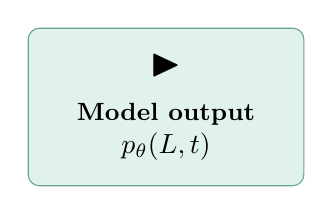
\begin{tikzpicture}
\node[
    rounded corners=4pt,
    draw=accentgreen!70,
    fill=softgreen,
    minimum width=3.5cm,
    minimum height=2.0cm,
    align=center
] {
    \Large $\blacktriangleright$\\[0.15cm]
    \small \textbf{Model output}\\
    $p_{\theta}(L,t)$
};
\end{tikzpicture}

\vspace{0.25cm}

{\scriptsize
Sound generated by the model\\
for parameters $\theta$.
}

\end{columns}


% -------------------------------------------------------------------------
% INVERSE PROBLEM — appears after the question
% -------------------------------------------------------------------------

\only<2->{

\vspace{0.15cm}

\centering

The calibration problem can then be written as

\vspace{-0.50cm}

\[
\boxed{
\theta^\star
=
\underset{\theta}{\operatorname{argmin}}
\;
\mathcal L
\left(
p_{\theta}(L,t),
p_{\mathrm{target}}(t)
\right)
}
\]

\vspace{-0.15cm}

{\small
Find the physical parameters whose simulated sound
is closest to the observation.
}

}

\end{frame}

% =============================================================================
% NUMERICAL SOLVER — MAIN PRESENTATION
% =============================================================================
\begin{frame}{Numerical Solver}

\begin{columns}[T,onlytextwidth]

% -------------------------------------------------------------------------
% LEFT COLUMN
% -------------------------------------------------------------------------
\column{0.43\textwidth}

\small

\textbf{Numerical strategy}

\vspace{0.25cm}

The coupled reed--acoustic model is solved using:

\vspace{0.15cm}

\begin{itemize}
    \setlength{\itemsep}{0.22cm}

    \item \textbf{Discontinuous Galerkin method}
    for the acoustic PDE;

    \item \textbf{Rusanov numerical flux}
    between neighbouring elements;

    \item \textbf{Characteristic variables}
    to impose the boundary conditions;

    \item \textbf{Explicit RK2 scheme}
    for time integration;

    \item \textbf{Damped Newton method}
    for the nonlinear reed boundary condition.

\end{itemize}

% -------------------------------------------------------------------------
% RIGHT COLUMN
% -------------------------------------------------------------------------
\column{0.53\textwidth}

\centering

\vspace{0.15cm}

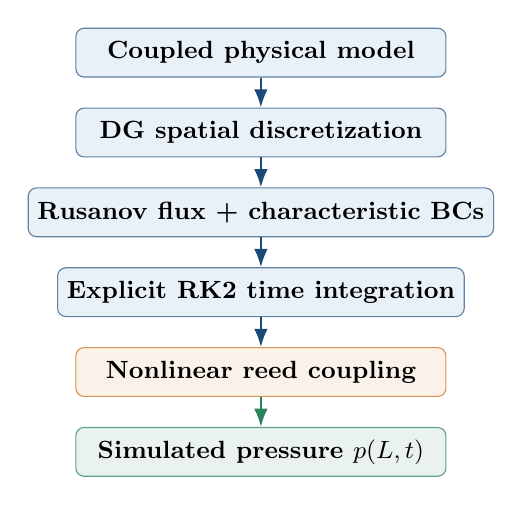
\begin{tikzpicture}[
    node distance=0.38cm,
    >=Latex,
    box/.style={
        rounded corners=3pt,
        draw=mainblue!70,
        fill=lightblue,
        minimum width=4.7cm,
        minimum height=0.62cm,
        align=center,
        font=\small\bfseries
    }
]

\node[box] (model)
{Coupled physical model};

\node[box,below=of model] (dg)
{DG spatial discretization};

\node[box,below=of dg] (bc)
{Rusanov flux + characteristic BCs};

\node[box,below=of bc] (rk)
{Explicit RK2 time integration};

\node[
    box,
    below=of rk,
    draw=accentorange!80,
    fill=accentorange!10
] (newton)
{Nonlinear reed coupling};

\node[
    box,
    below=of newton,
    draw=accentgreen!75,
    fill=accentgreen!10
] (signal)
{Simulated pressure $p(L,t)$};

\draw[->,thick,mainblue] (model)--(dg);
\draw[->,thick,mainblue] (dg)--(bc);
\draw[->,thick,mainblue] (bc)--(rk);
\draw[->,thick,mainblue] (rk)--(newton);
\draw[->,thick,accentgreen] (newton)--(signal);

\end{tikzpicture}

\vspace{0.25cm}

\greenbox{0.94\linewidth}{
\small
Implemented in \textbf{JAX} as a fully
differentiable numerical solver.
}

\end{columns}

\end{frame}
% =============================================================================
% 5. VALIDATION AND PERFORMANCE
% =============================================================================
\begin{frame}{Forward Solver Validation}
\vspace{-0.15cm}

\begin{columns}[T,onlytextwidth]

% =========================================================================
% LEFT COLUMN : SIGNAL COMPARISONS
% =========================================================================
\column{0.49\textwidth}

\textbf{\color{mainblue}Comparison with OpenWind}
\footnotemark[1]

\vspace{-0.15cm}

\begin{center}
    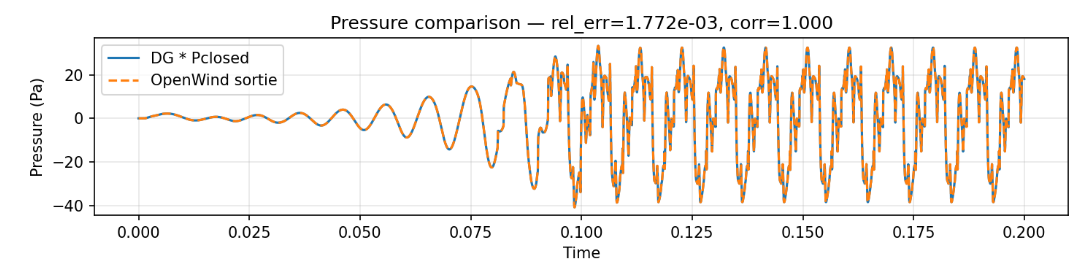
\includegraphics[
        width=0.96\linewidth,
        keepaspectratio
    ]{../Images/press_compare_const.png}

    \vspace{-0.10cm}

    {\scriptsize Constant-section resonator}
\end{center}

\vspace{-0.35cm}

\begin{center}
    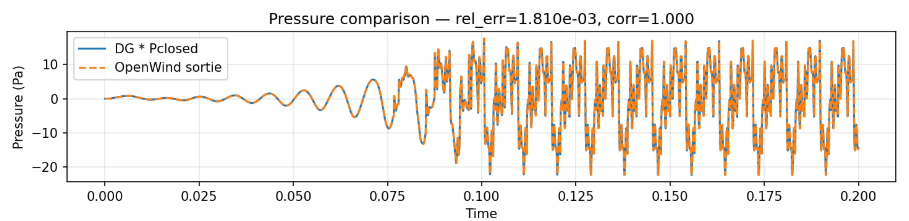
\includegraphics[
        width=0.96\linewidth,
        keepaspectratio
    ]{../Images/press_compare_exp.png}

    \vspace{-0.10cm}

    {\scriptsize Exponential-section resonator}
\end{center}

\vspace{-0.15cm}

\bluebox{0.94\linewidth}{
\small
Good agreement between the DG solver
and OpenWind for different resonator geometries.
}


% =========================================================================
% RIGHT COLUMN : CONVERGENCE
% =========================================================================
\column{0.49\textwidth}

\textbf{\color{mainblue}Mesh convergence}

For proportional mesh refinement, second-order accuracy predicts

\vspace{-0.25cm}
\[
\boxed{
\|u_h^{\mathrm{DG}}-u_\eta^{\mathrm{OW}}\|
=
\mathcal O(h^2),
\qquad \eta\propto h.
}
\]

\begin{center}

    % Replace by your convergence figure
    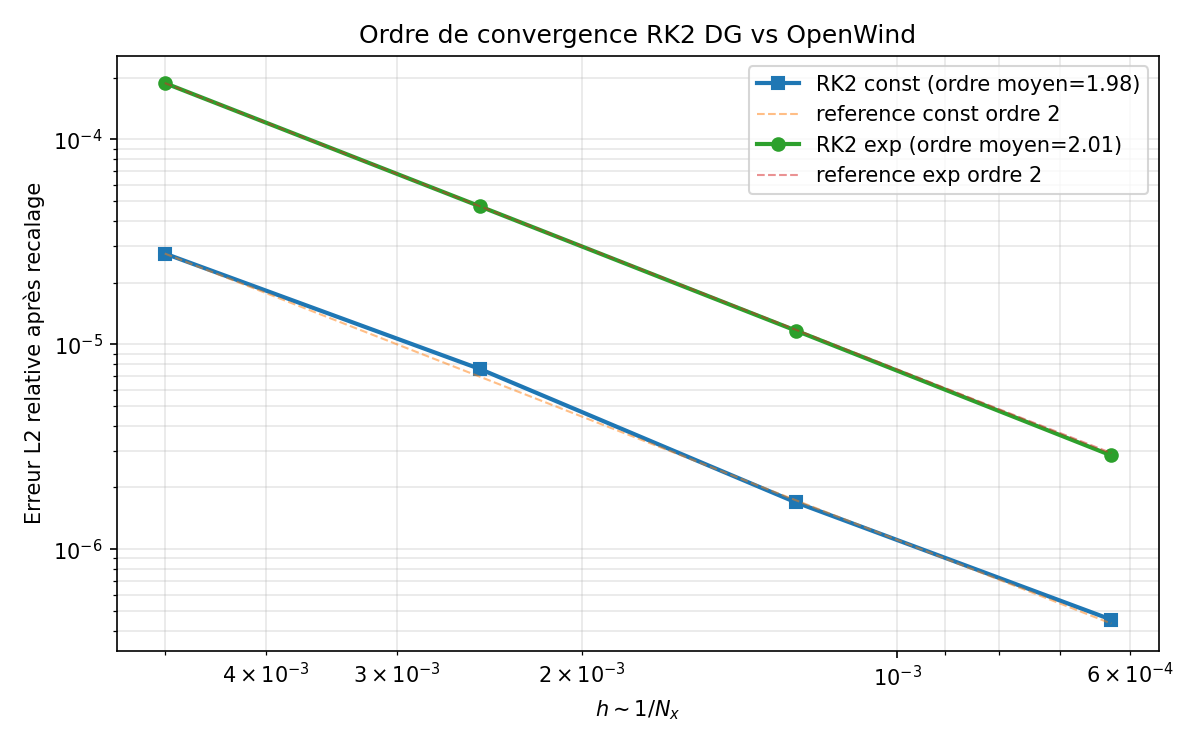
\includegraphics[
        width=0.95\linewidth,
        keepaspectratio
    ]{../../experiments/convergence/results/convergence_compare_shift_rk2.png}

    \vspace{-0.25cm}

    {\scriptsize
    Relative error between DG and OpenWind
    as the spatial mesh is refined.
    }

\end{center}

\end{columns}


\footnotetext[1]{
{\footnotesize
\cite{OpenwindInria}
OpenWind -- INRIA.
}
}

\end{frame}

% =============================================================================
% DIFFERENTIABLE SOLVER
% =============================================================================
\begin{frame}{Differentiable Solver \footnotemark[1]}
\vspace{-0.15cm}
\begin{columns}[T,onlytextwidth]

% -------------------------------------------------------------------------
% LEFT COLUMN
% -------------------------------------------------------------------------
\column{0.5\textwidth}

\small

\textbf{From simulation to calibration}

\vspace{0.10cm}

Two sets of unknowns can be considered:
\vspace{-0.25cm}
\[
\underbrace{\theta}_{\text{physical parameters}}
=
(\gamma,\kappa,\zeta,\ldots),
\]
\vspace{-0.25cm}
\[
\underbrace{\eta}_{\text{NN parameters}},
\qquad
\ell_\eta(y)
\simeq
\ell(y).
\]

\vspace{-0.15cm}

The numerical solver therefore defines
\vspace{-0.15cm}
\[
(\theta,\eta)
\longmapsto
p_{\theta,\eta}(L,t).
\]

\vspace{-0.15cm}

Implemented in \textbf{JAX}\footnotemark[2] to enable automatic differentiation through 
the numerical solver (wherever the implemented operations are differentiable with respect 
to the calibrated parameters):

\vspace{-0.15cm}
\[
\boxed{
\nabla_{\theta,\eta}
\mathcal L
\left(
p_{\theta,\eta},
p_{\mathrm{target}}
\right)
}
\]

% -------------------------------------------------------------------------
% RIGHT COLUMN
% -------------------------------------------------------------------------
\column{0.5\textwidth}

\vspace{-0.2cm}

providing gradients for both
\textbf{physical calibration} and
\textbf{reed-law identification}.

\centering

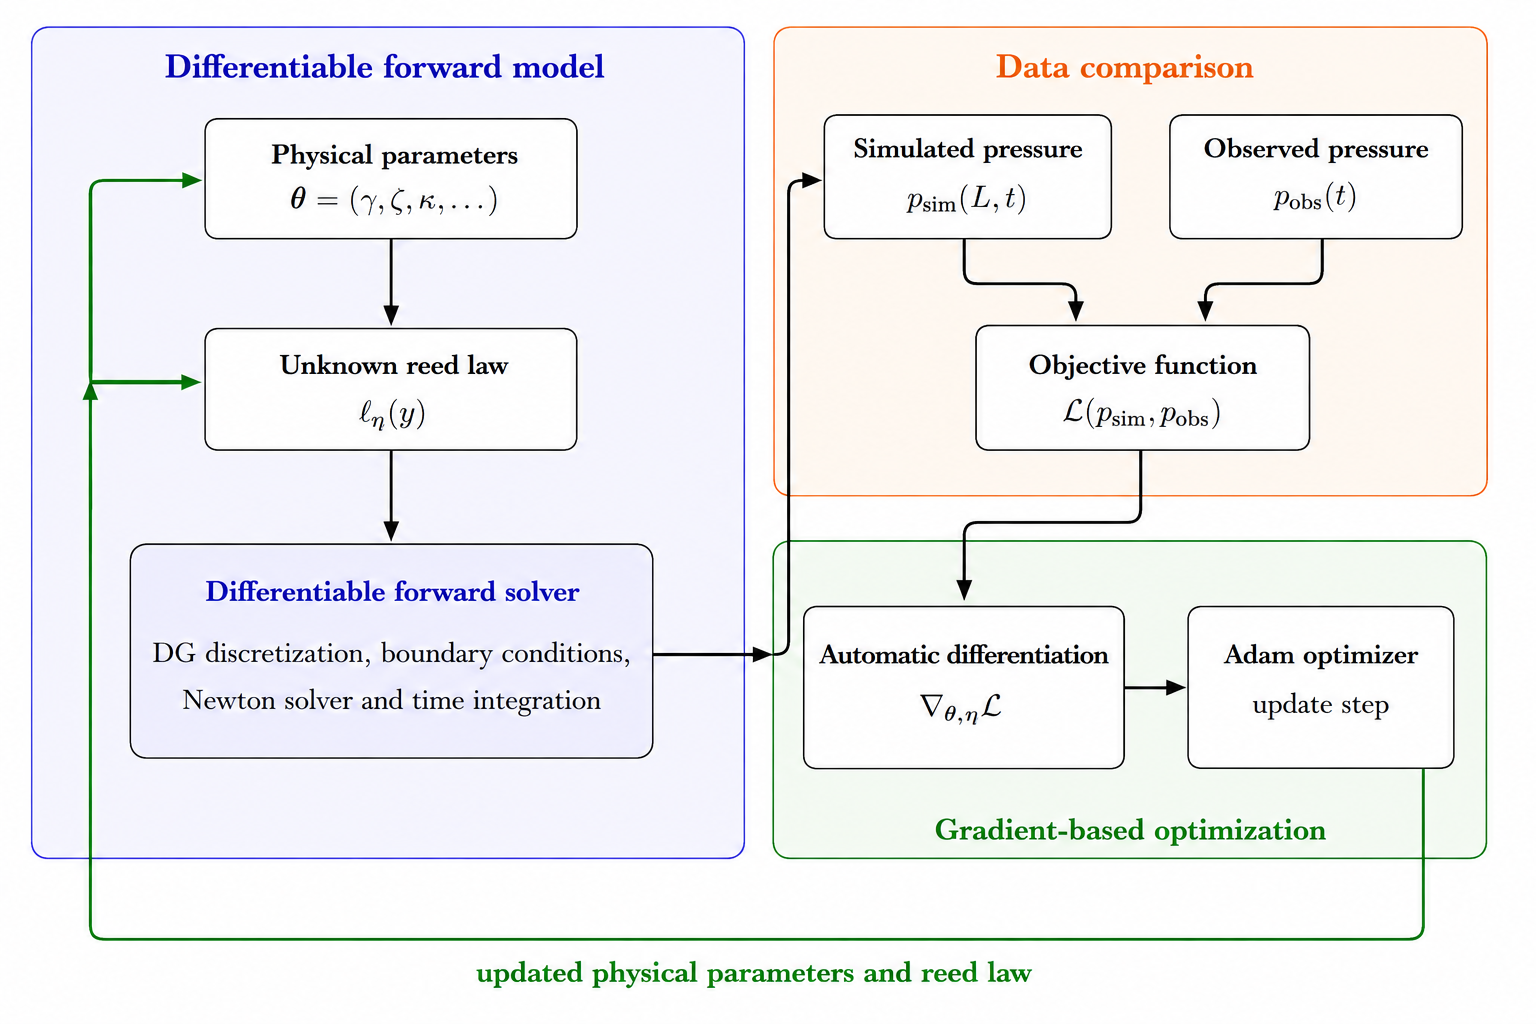
\includegraphics[
    width=\linewidth
]{../Images/pipeline_diff_auto.png}

{\scriptsize
Differentiable simulation and gradient-based optimization pipeline.
}

\end{columns}

\footnotetext[1]{
{\footnotesize \cite{griewank2008evaluating}
Griewank, Andreas and Walther, Andrea (2008), \emph{Evaluating Derivatives: Principles and Techniques of Algorithmic Differentiation}}
}

\footnotetext[2]{
{\footnotesize \cite{jax_autodiff}
\url{https://docs.jax.dev/en/latest/jacobian-vector-products.html}}
}

\end{frame}

% =============================================================================
% MULTI-SCALE SPECTRAL LOSS
% =============================================================================
\begin{frame}{Multi-Scale Spectral Loss}

\vspace{-0.25cm}

\begin{columns}[T,onlytextwidth]

% =========================================================================
% LEFT COLUMN : ONE STFT RESOLUTION
% =========================================================================
\column{0.48\textwidth}

\small

\textbf{\color{mainblue}Short-Time Fourier Transform (STFT)}
\footnotemark[1]

\vspace{-0.05cm}

For a given resolution

\vspace{-0.25cm}
\[
\boxed{
r=(N_r,H_r)
}
\]

where $N_r$ is the window size and $H_r$ the hop size,
the STFT of a signal $x$ is

\vspace{-0.60cm}
\[
\boxed{
X^{(r)}(m,k)
=
\sum_n
x[n]\,
w_r[n-mH_r]\,
e^{-i2\pi kn/N_r}
}
\]

\vspace{-0.6cm}

\begin{center}
    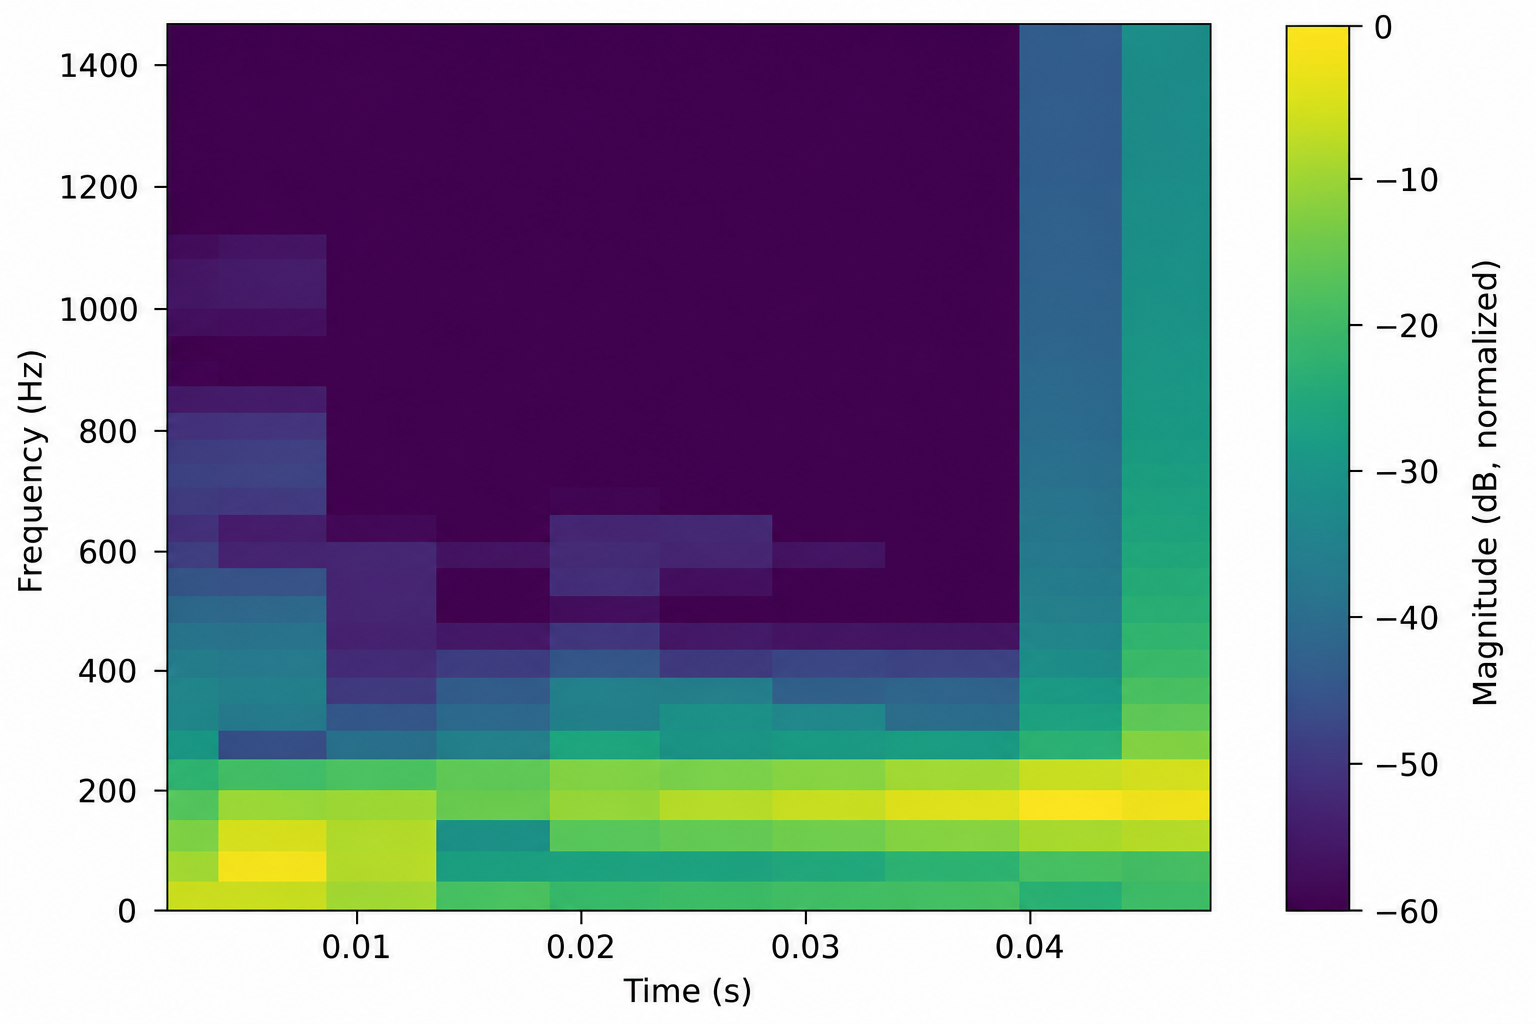
\includegraphics[
        width=0.7\linewidth,
        keepaspectratio
    ]{../Images/spectro_example.png}

    \vspace{-0.25cm}
    {\scriptsize
    STFT magnitude: time--frequency representation.
    }
\end{center}



% =========================================================================
% RIGHT COLUMN : MULTI-SCALE LOSS
% =========================================================================
\column{0.48\textwidth}

\small

\textbf{\color{mainblue}Multi-Scale Spectral Loss}
\footnotemark[2]

Since each resolution produces a different
time-frequency representation, we use several resolutions:

\vspace{-0.6cm}
\[
\mathcal R =
\left\{
(64,16),
(128,32),
(256,64),
(512,128)
\right\}.
\]

\vspace{-0.2cm}

\bluebox{0.94\linewidth}{
\small
Short windows provide better temporal resolution,
while long windows provide better frequency resolution.
}


\[
\begin{array}{ccc}
p_\theta
&
\xrightarrow{\mathrm{STFT}_r}
&
|X_\theta^{(r)}|
\\[0.15cm]
p_{\rm target}
&
\xrightarrow{\mathrm{STFT}_r}
&
|X_{\rm target}^{(r)}|
\end{array}
\]

\[
\mathcal L_{\rm STFT}^{(r)}
=
\mathcal D
\left(
|X_\theta^{(r)}|,
|X_{\rm target}^{(r)}|
\right).
\]

\vspace{-0.15cm}
\[
\boxed{
\mathcal L_{\rm MSTS}
=
\frac{1}{|\mathcal R|}
\sum_{r\in\mathcal R}
\mathcal L_{\rm STFT}^{(r)}
}
\]
\end{columns}


% =========================================================================
% FOOTNOTES
% =========================================================================
\footnotetext[1]{
{\footnotesize
\cite{allen1977stft}
Allen, J. B. and Rabiner, L. R. (1977),
\emph{A Unified Approach to Short-Time Fourier Analysis and Synthesis}.
}
}

\footnotetext[2]{
{\footnotesize
\cite{schwaer2023multi}
Schwär, S. and Müller, M. (2023),
\emph{Multi-Scale Spectral Loss Revisited}.
}
}

\end{frame}

% =============================================================================
% 7. CALIBRATION PROTOCOL
% =============================================================================
\begin{frame}{Calibration Protocol}

  \begin{center}
        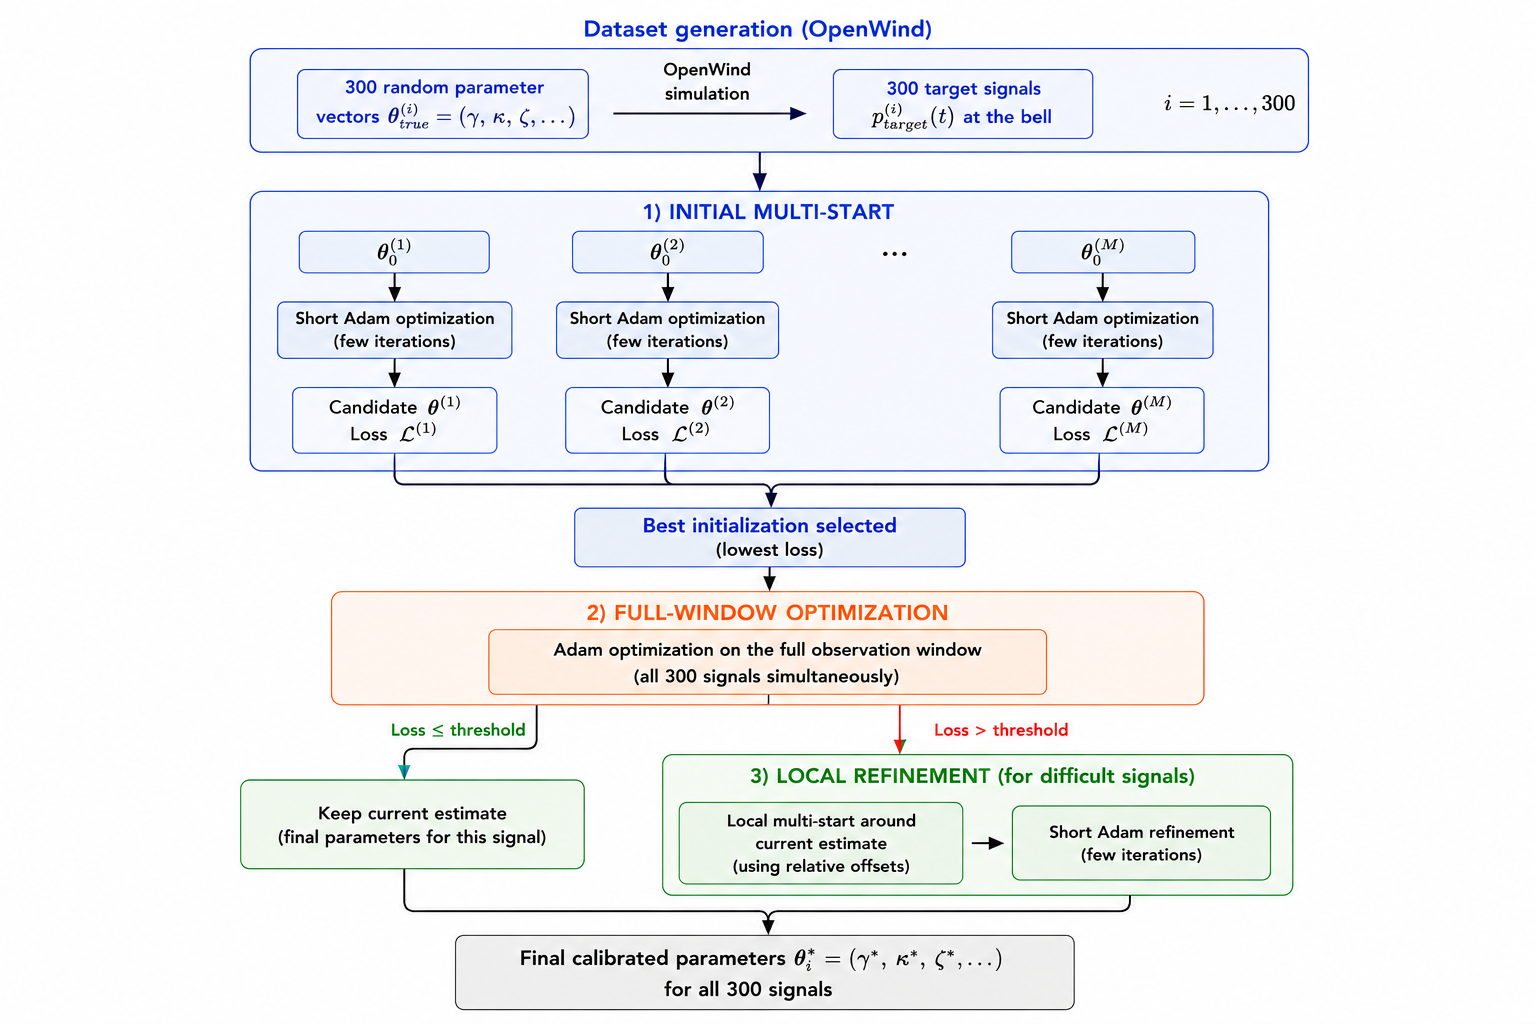
\includegraphics[width=0.7\linewidth,keepaspectratio]{../Images/pipeline_calibration_simplified.png}\hspace{0.0em}%
        \par\smallskip
        \scriptsize Pipeline for the total calibration process.
        \label{fig:pipeline_calibration_simplified}  
  \end{center}
\end{frame}

% =============================================================================
% BACKWARD PERFORMANCE
% =============================================================================
\begin{frame}{Computational Cost of Reverse-Mode Differentiation}

\vspace{-0.2cm}
\begin{columns}[T,onlytextwidth]

% -------------------------------------------------------------------------
% LEFT COLUMN
% -------------------------------------------------------------------------
\column{0.62\textwidth}

\centering

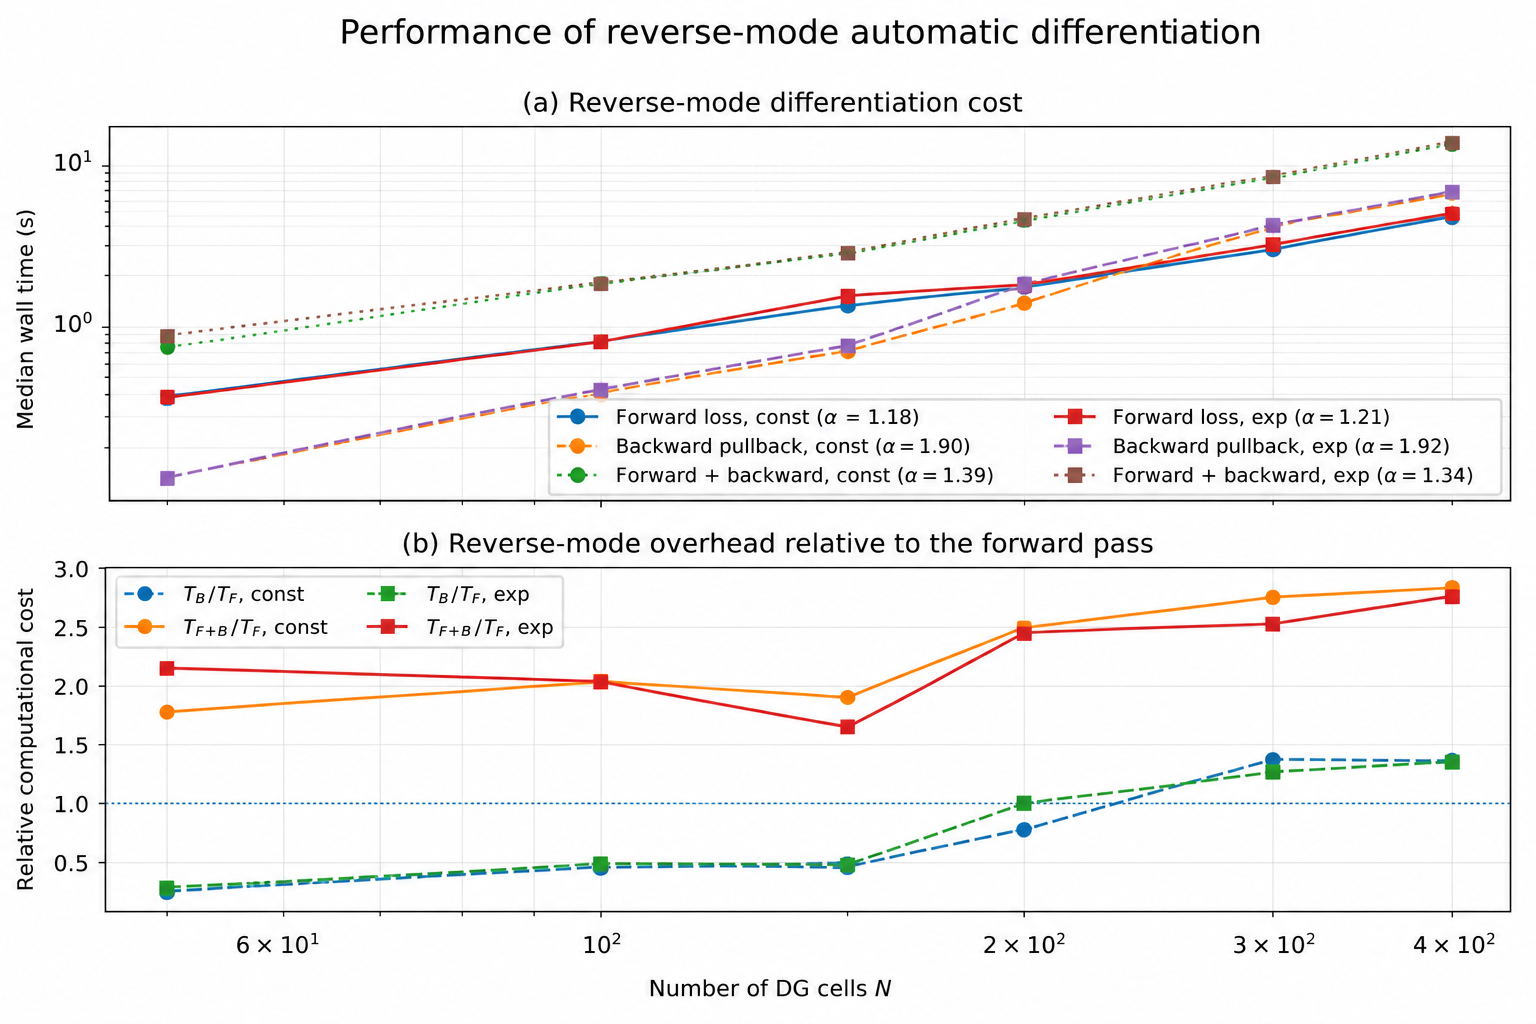
\includegraphics[
    width=1.0\linewidth
]{../../experiments/performance/results_backward/performance_backward_summary_rk2_small.png}

{\scriptsize
Performance of reverse-mode differentiation for the RK2 + Newton solver
as a function of the number of DG elements $N$.
}

% -------------------------------------------------------------------------
% RIGHT COLUMN
% -------------------------------------------------------------------------
\column{0.34\textwidth}

\small

\textbf{Main observations}

\vspace{0.15cm}

\bluebox{0.96\linewidth}{
\small
For small and intermediate meshes,
the backward pass costs
\textbf{less than one forward evaluation}.
}

\vspace{0.18cm}

\greenbox{0.96\linewidth}{
\small
Over the tested range, a complete
\textbf{forward + backward}
evaluation costs only about
\[
1.8\text{--}2.8\times
\]
one forward simulation.
}

\vspace{0.18cm}

\orangebox{0.96\linewidth}{
\small
A single backward pass provides
gradients with respect to
\textbf{all calibrated parameters}
simultaneously, making reverse-mode AD
well suited to inverse calibration.
}

\vspace{0.15cm}

\end{columns}

\end{frame}



% =============================================================================
% 8. PARAMETER RESULTS
% =============================================================================
\begin{frame}{Parameter Calibration Results}
\begin{columns}[T,onlytextwidth]
\column{0.57\textwidth}
\vspace{-0.25cm}
\textbf{Main calibrated parameters}
\vspace{-0.2cm}
\begin{center}
        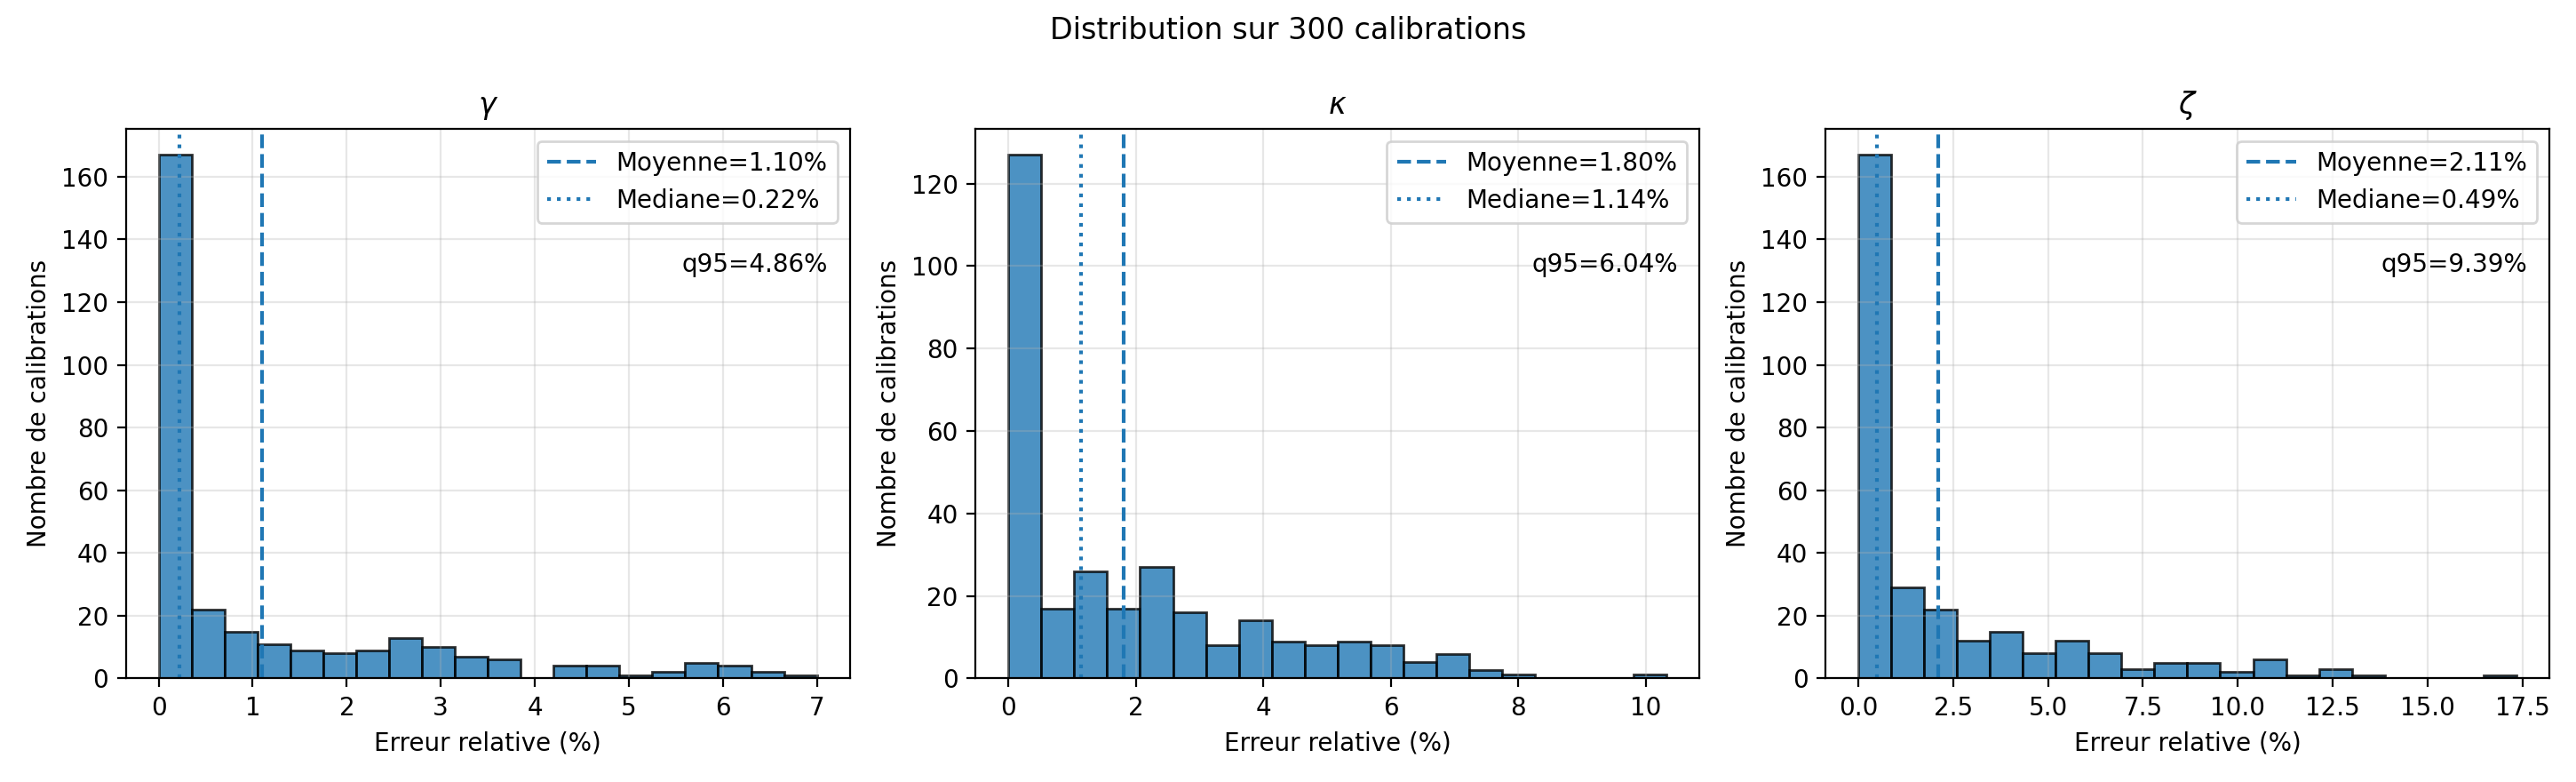
\includegraphics[width=1.0\linewidth,keepaspectratio]{../../experiments/gradient/results/gamma_kappa_zeta_Qr_fixed_pressure_only/error_histograms.png}\hspace{0.0em}%
        \par\smallskip
        \scriptsize Comparison of the calibrated parameters with the ground truth on noise-free synthetic data.
        \label{fig:error_histograms}  
    \end{center}
\vspace{-0.05cm}
\greenbox{0.96\linewidth}{Accurate recovery of the main reed parameters on noise-free synthetic data.}

\column{0.39\textwidth}
\vspace{-0.25cm}
\textbf{Spectrogram comparison}
\vspace{-0.2cm}
\begin{center}
        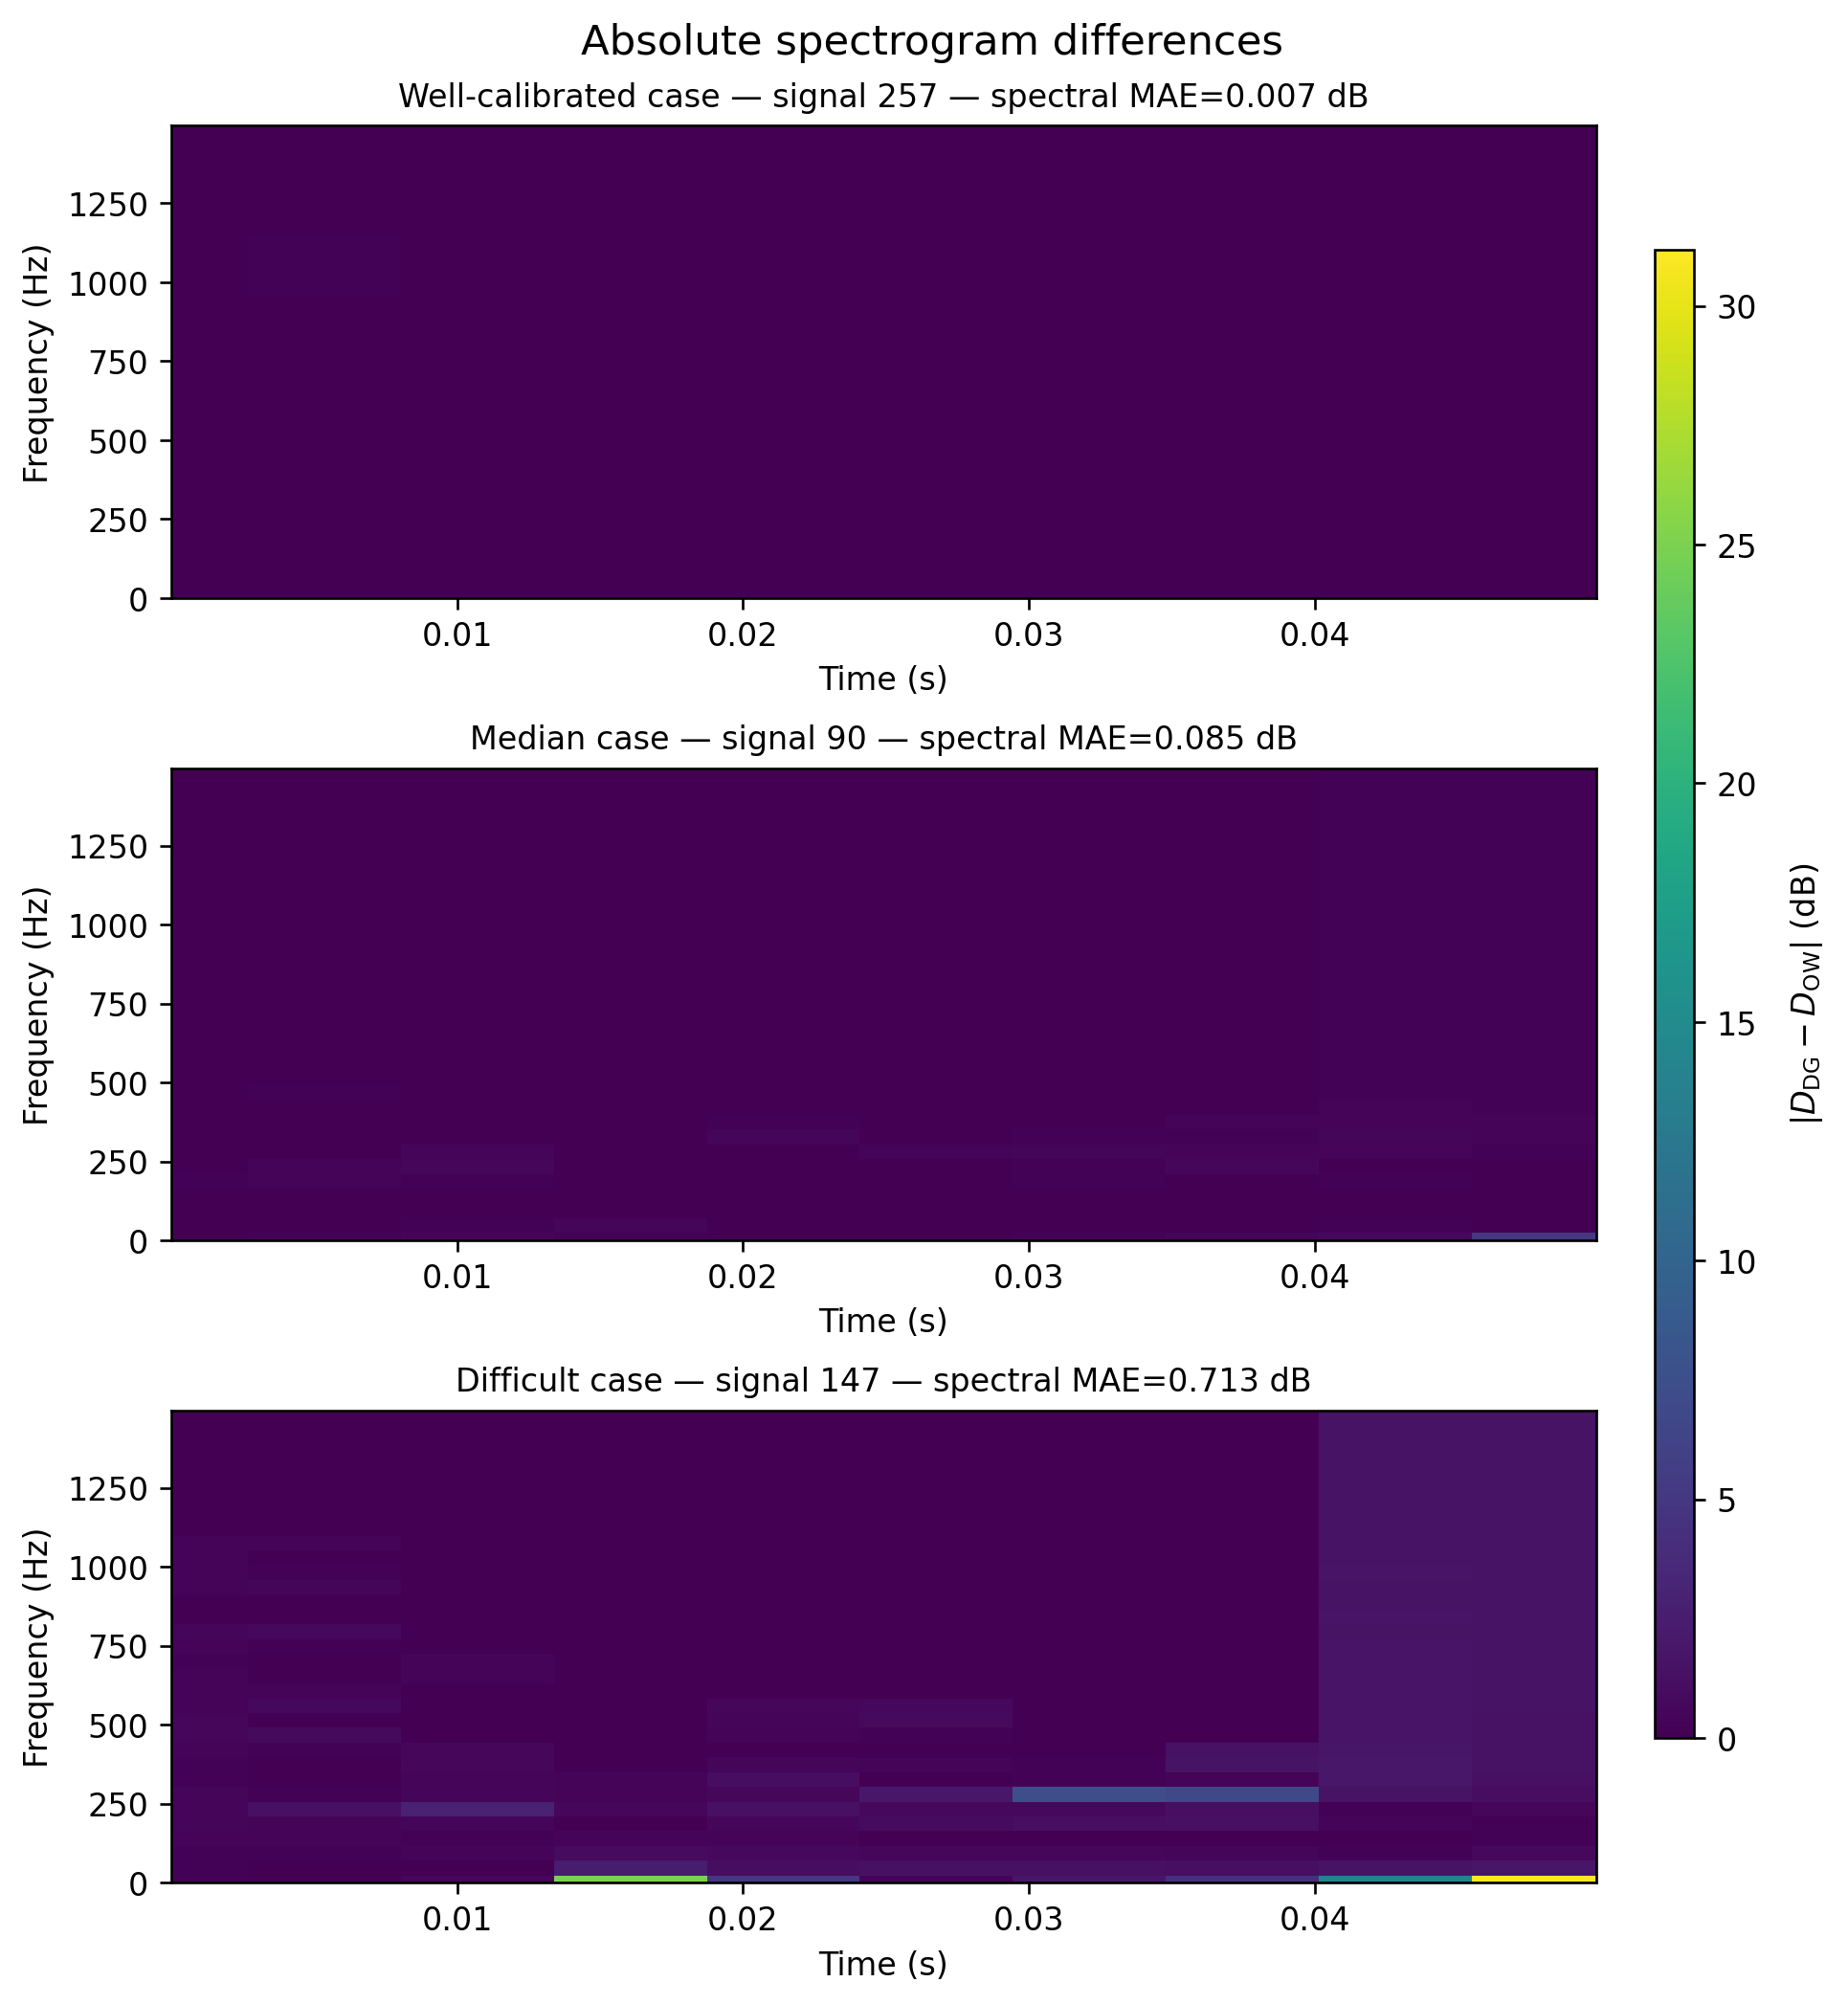
\includegraphics[width=0.7\linewidth,keepaspectratio]{../../experiments/gradient/results/representative_calibration_spectrograms/representative_spectrogram_differences.png}\hspace{0.0em}%
        \par\smallskip
        \scriptsize Comparison of the spectrograms of the calibrated and target signals.
        \label{fig:representative_spectrogram_differences}  
    \end{center}
\vspace{0.05cm}
\end{columns}
\vspace{-0.3cm}
\orangebox{0.96\linewidth}{
%
\begin{minipage}[c]{0.52\linewidth}
    Mean absolute spectral error (dB) : 
    \vspace{-0.5cm}
    \centering

    \[
    E_{\mathrm{dB}}
    =
    \frac{1}{N_{\mathrm{TF}}}
    \sum_{m,k}
    \left|
    D^{\mathrm{DG}}(m,k)
    -
    D^{\mathrm{OW}}(m,k)
    \right|
    \]

\end{minipage}
\hfill
\begin{minipage}[c]{0.43\linewidth}

    \scriptsize

    $D^{\mathrm{OW}}(m,k)$:
    log-magnitude spectrogram of the target signal.

    \vspace{0.12cm}

    $D^{\mathrm{DG}}(m,k)$:
    log-magnitude spectrogram of the calibrated signal.

    \vspace{0.12cm}

    $N_{\mathrm{TF}}$:
    total number of time--frequency coefficients.

\end{minipage}
}
\end{frame}

% =============================================================================
% LISTENING COMPARISON
% =============================================================================
\begin{frame}{Listening Comparison}

\centering

\small
Same OpenWind model, with three different parameter sets.

\vspace{0.45cm}

\begin{columns}[c,onlytextwidth]

% =========================================================================
% INITIAL PARAMETERS
% =========================================================================
\column{0.31\textwidth}
\centering

\textattachfile[
    mimetype=audio/mpeg,
    description={OpenWind sound with initial parameters},
    color=0 0 1
]{01_initial_parameters_openwind.wav}{%
    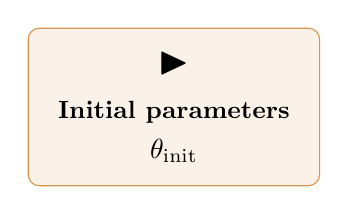
\begin{tikzpicture}
    \node[
        rounded corners=4pt,
        draw=accentorange!80,
        fill=accentorange!10,
        minimum width=3.7cm,
        minimum height=2.0cm,
        align=center
    ] {
        \Large $\blacktriangleright$\\[0.15cm]
        \small \textbf{Initial parameters}\\[0.08cm]
        $\theta_{\rm init}$
    };
    \end{tikzpicture}%
}

\vspace{0.15cm}

{\scriptsize Before calibration}


% =========================================================================
% CALIBRATED PARAMETERS
% =========================================================================
\column{0.31\textwidth}
\centering

\textattachfile[
    mimetype=audio/mpeg,
    description={OpenWind sound with calibrated parameters},
    color=0 0 1
]{02_calibrated_parameters_openwind.wav}{%
    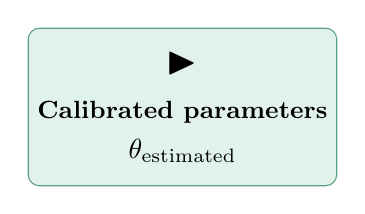
\begin{tikzpicture}
    \node[
        rounded corners=4pt,
        draw=accentgreen!75,
        fill=softgreen,
        minimum width=3.7cm,
        minimum height=2.0cm,
        align=center
    ] {
        \Large $\blacktriangleright$\\[0.15cm]
        \small \textbf{Calibrated parameters}\\[0.08cm]
        $\theta_{\rm estimated}$
    };
    \end{tikzpicture}%
}

\vspace{0.15cm}

{\scriptsize After calibration}


% =========================================================================
% TRUE PARAMETERS
% =========================================================================
\column{0.31\textwidth}
\centering

\textattachfile[
    mimetype=audio/mpeg,
    description={OpenWind reference sound with true parameters},
    color=0 0 1
]{03_true_parameters_openwind.wav}{%
    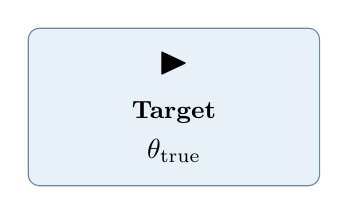
\begin{tikzpicture}
    \node[
        rounded corners=4pt,
        draw=mainblue!65,
        fill=lightblue,
        minimum width=3.7cm,
        minimum height=2.0cm,
        align=center
    ] {
        \Large $\blacktriangleright$\\[0.15cm]
        \small \textbf{Target}\\[0.08cm]
        $\theta_{\rm true}$
    };
    \end{tikzpicture}%
}

\vspace{0.15cm}

{\scriptsize Reference sound}

\end{columns}


% =========================================================================
% INTERPRETATION
% =========================================================================

\vspace{0.55cm}

\greenbox{0.90\linewidth}{
\small
The calibrated parameters produce a sound
very close to the reference.
}

\vspace{0.25cm}

{\scriptsize\color{gray}
For this listening comparison, all three sounds are generated with OpenWind;
only the parameter values are changed.
}

\end{frame}

% =============================================================================
% 9. L(Y)
% =============================================================================
\begin{frame}{Learning the Reed Opening Law $\ell(y)$}
    \vspace{-0.15cm}
    \textbf{Beyond scalar parameters}
    \vspace{-0.15cm}
    \begin{columns}[T,onlytextwidth]
    \column{0.7\textwidth}
    \begin{center}
        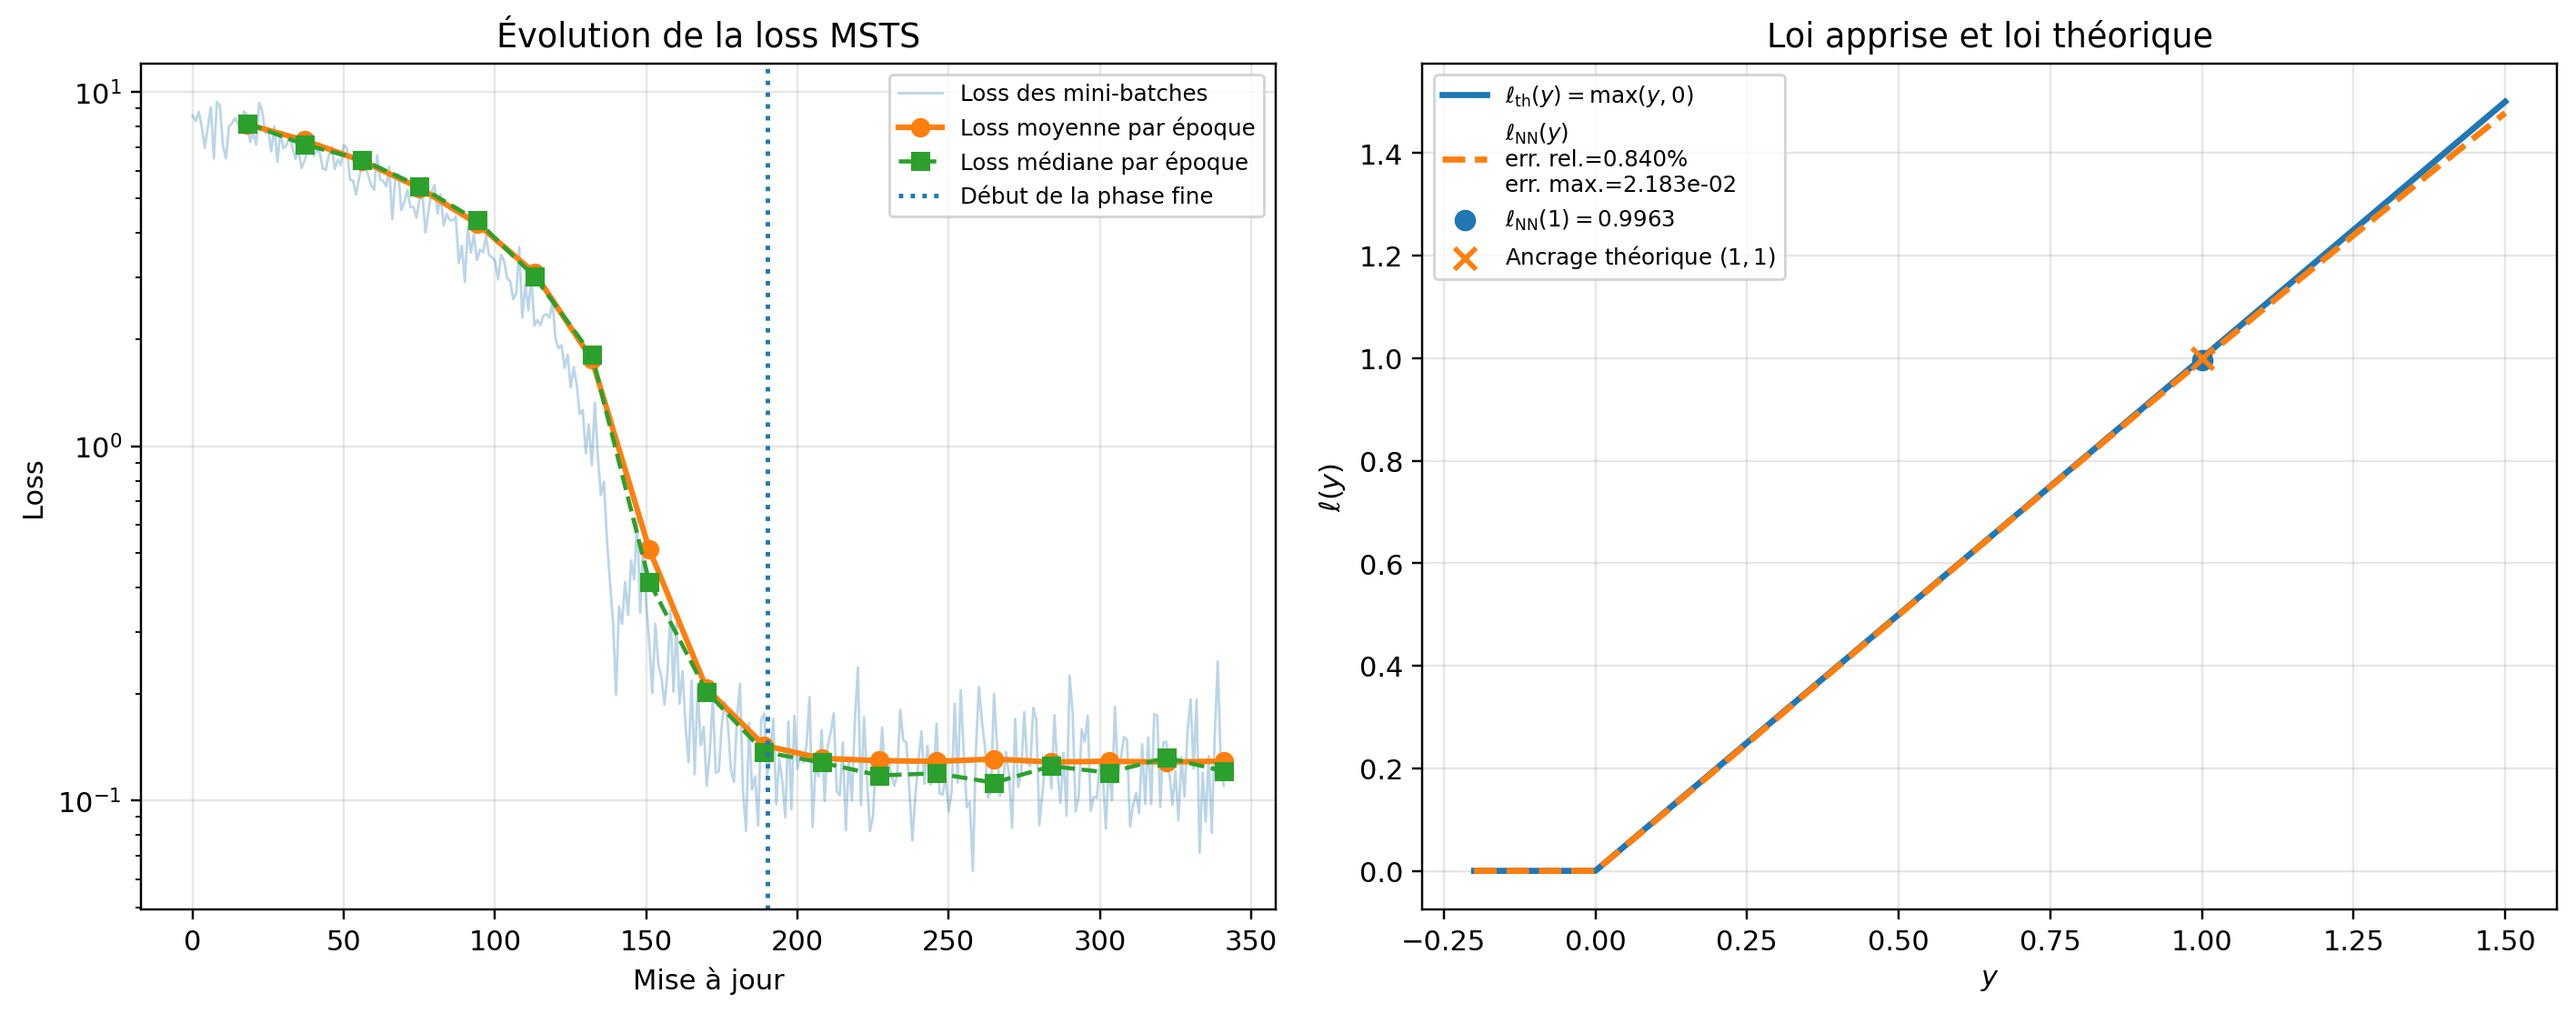
\includegraphics[width=1.0\linewidth,keepaspectratio]{../../experiments/gradient/results/train_l_only_msts_openwind_matched/clean/training_summary.png}\hspace{0.0em}%
        \par\smallskip
        \scriptsize Training of the neural network $\ell_\eta(y)$ to match the target law $\ell(y)=\max(y,0)$.
        \label{fig:training_summary}  
    \end{center}
    \column{0.28\textwidth}
    \vspace{0.6cm}
    \begin{itemize}
        \item Neural network: $[1,8,8,1]$ with $\tanh$ activation.
        \item Anchoring points: $\ell(1)=1$.
        \item \small Example result: relative error below $1\%$ in the synthetic setting.
    \end{itemize}
    \end{columns}
\vspace{0.5cm}

\greenbox{0.95\linewidth}{The framework extends from parameter calibration to model-law identification.}

\end{frame}

% =============================================================================
% 10. NOISE
% =============================================================================
% =============================================================================
% NOISE MODEL
% =============================================================================
\begin{frame}{Noise Model}

\begin{columns}[T,onlytextwidth]

% -------------------------------------------------------------------------
% LEFT COLUMN
% -------------------------------------------------------------------------
\column{0.48\textwidth}

\small

\textbf{Noisy observation}

\vspace{0.2cm}

Starting from a clean OpenWind target signal
$p_{\rm clean}(t)$, we construct

\[
p_{\rm noisy}(t)
=
p_{\rm clean}(t)
+
n(t),
\]

where $n(t)$ is additive white Gaussian noise.

\vspace{0.25cm}

The noise amplitude is adjusted to obtain a prescribed
signal-to-noise ratio:

\[
\boxed{
\mathrm{SNR}
=
10\log_{10}
\left(
\frac{\|p_{\rm clean}\|_2^2}
     {\|n\|_2^2}
\right)
}
\]

\vspace{0.25cm}

The calibration is repeated for

\[
\mathrm{SNR}
\in
\{40,30,20,10\}\ \mathrm{dB}.
\]


% -------------------------------------------------------------------------
% RIGHT COLUMN
% -------------------------------------------------------------------------
\column{0.48\textwidth}

\centering

\textbf{Experimental protocol}

\vspace{0.25cm}

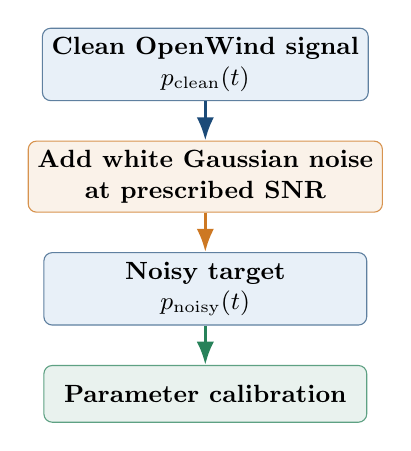
\begin{tikzpicture}[
    node distance=0.5cm,
    >=Latex
]

\tikzset{
    b/.style={
        rounded corners=3pt,
        draw=mainblue!70,
        fill=lightblue,
        minimum width=4.1cm,
        minimum height=0.72cm,
        align=center,
        font=\small\bfseries
    }
}

\node[b] (clean)
{Clean OpenWind signal\\$p_{\rm clean}(t)$};

\node[
    b,
    below=of clean,
    fill=accentorange!10,
    draw=accentorange!80
] (noise)
{Add white Gaussian noise\\at prescribed SNR};

\node[
    b,
    below=of noise
] (target)
{Noisy target\\$p_{\rm noisy}(t)$};

\node[
    b,
    below=of target,
    fill=accentgreen!10,
    draw=accentgreen!75
] (calib)
{Parameter calibration};

\draw[->,very thick,mainblue]
(clean)--(noise);

\draw[->,very thick,accentorange]
(noise)--(target);

\draw[->,very thick,accentgreen]
(target)--(calib);

\end{tikzpicture}

\vspace{0.25cm}

\orangebox{0.95\linewidth}{
\small
The true physical parameters remain unchanged:
only the observation is corrupted by noise.
}

\end{columns}

\end{frame}

% =============================================================================
% ROBUSTNESS TO NOISE
% =============================================================================
\begin{frame}{Calibration under Noisy Observations}
\vspace{-0.2cm}
\begin{columns}[T,onlytextwidth]

% -------------------------------------------------------------------------
% LEFT COLUMN : overall behaviour
% -------------------------------------------------------------------------
\column{0.55\textwidth}

\textbf{Parameter recovery as a function of SNR}

\vspace{-0.2cm}
\begin{table}[htbp]
\centering
\label{tab:noisy_parameter_errors}
\scriptsize
\begin{tabular}{lccc}
\toprule
Observation condition
& \(\gamma\)
& \(\kappa\)
& \(\zeta\) \\
\midrule
Noise-free
& \(1.10\%\)
& \(1.80\%\)
& \(2.11\%\) \\
\(40\,\mathrm{dB}\)
& \(1.71\%\)
& \(2.61\%\)
& \(4.81\%\) \\
\(30\,\mathrm{dB}\)
& \(3.67\%\)
& \(4.79\%\)
& \(8.38\%\) \\
\(20\,\mathrm{dB}\)
& \(17.77\%\)
& \(13.85\%\)
& \(26.23\%\) \\
\(10\,\mathrm{dB}\)
& \(25.78\%\)
& \(19.91\%\)
& \(29.07\%\) \\
\bottomrule
\end{tabular}
\end{table}
\vspace{-0.45cm}
\begin{center}
        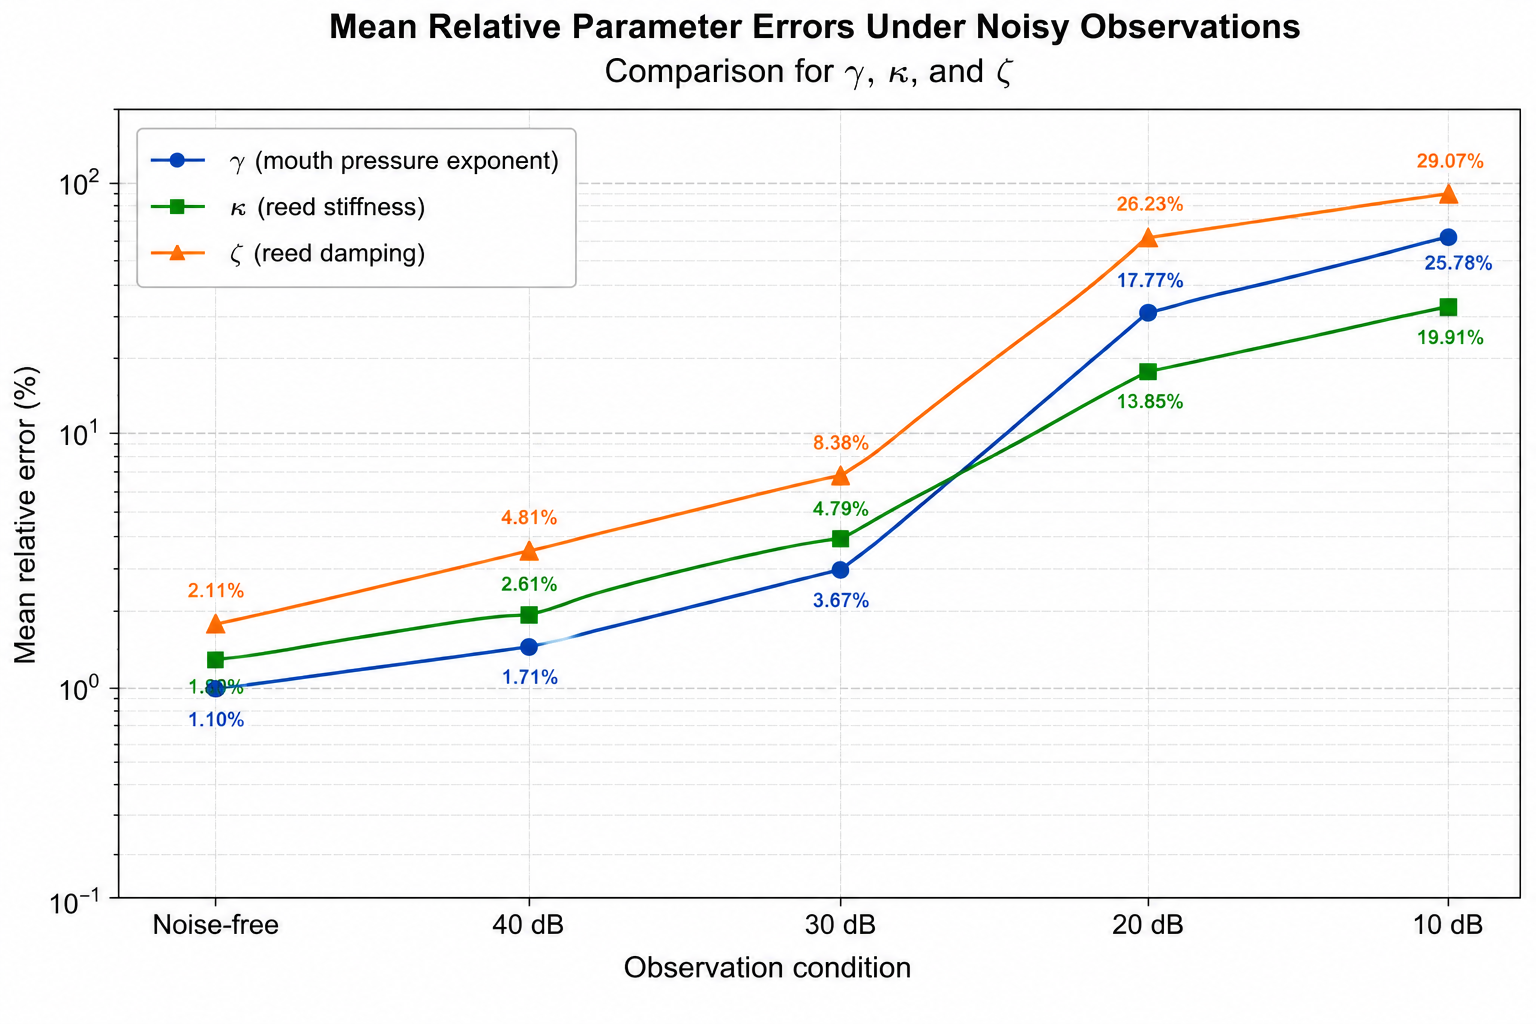
\includegraphics[width=0.85\linewidth,keepaspectratio]{../Images/relative_error_noisy.png}\hspace{0.0em}%
        \label{fig:relative_error_noisy}  
    \end{center}


% -------------------------------------------------------------------------
% RIGHT COLUMN : interpretation + 10 dB comparison
% -------------------------------------------------------------------------
\column{0.42\textwidth}

\small

\textbf{Main observation}

\begin{itemize}
    \item Calibration remains accurate at high SNR.
    \item Errors increase markedly below $30$ dB.
\end{itemize}

\vspace{-0.1cm}

\textbf{10 dB case} \tiny $(L_i,H_i)\in$

$\left\{
(64,32),
(128,64),
(256,128)
\right\}\rightarrow
\left\{
(64,16),
(128,32),
(256,64),
(512,128)
\right\}$

\vspace{-0.15cm}

\begin{center}
        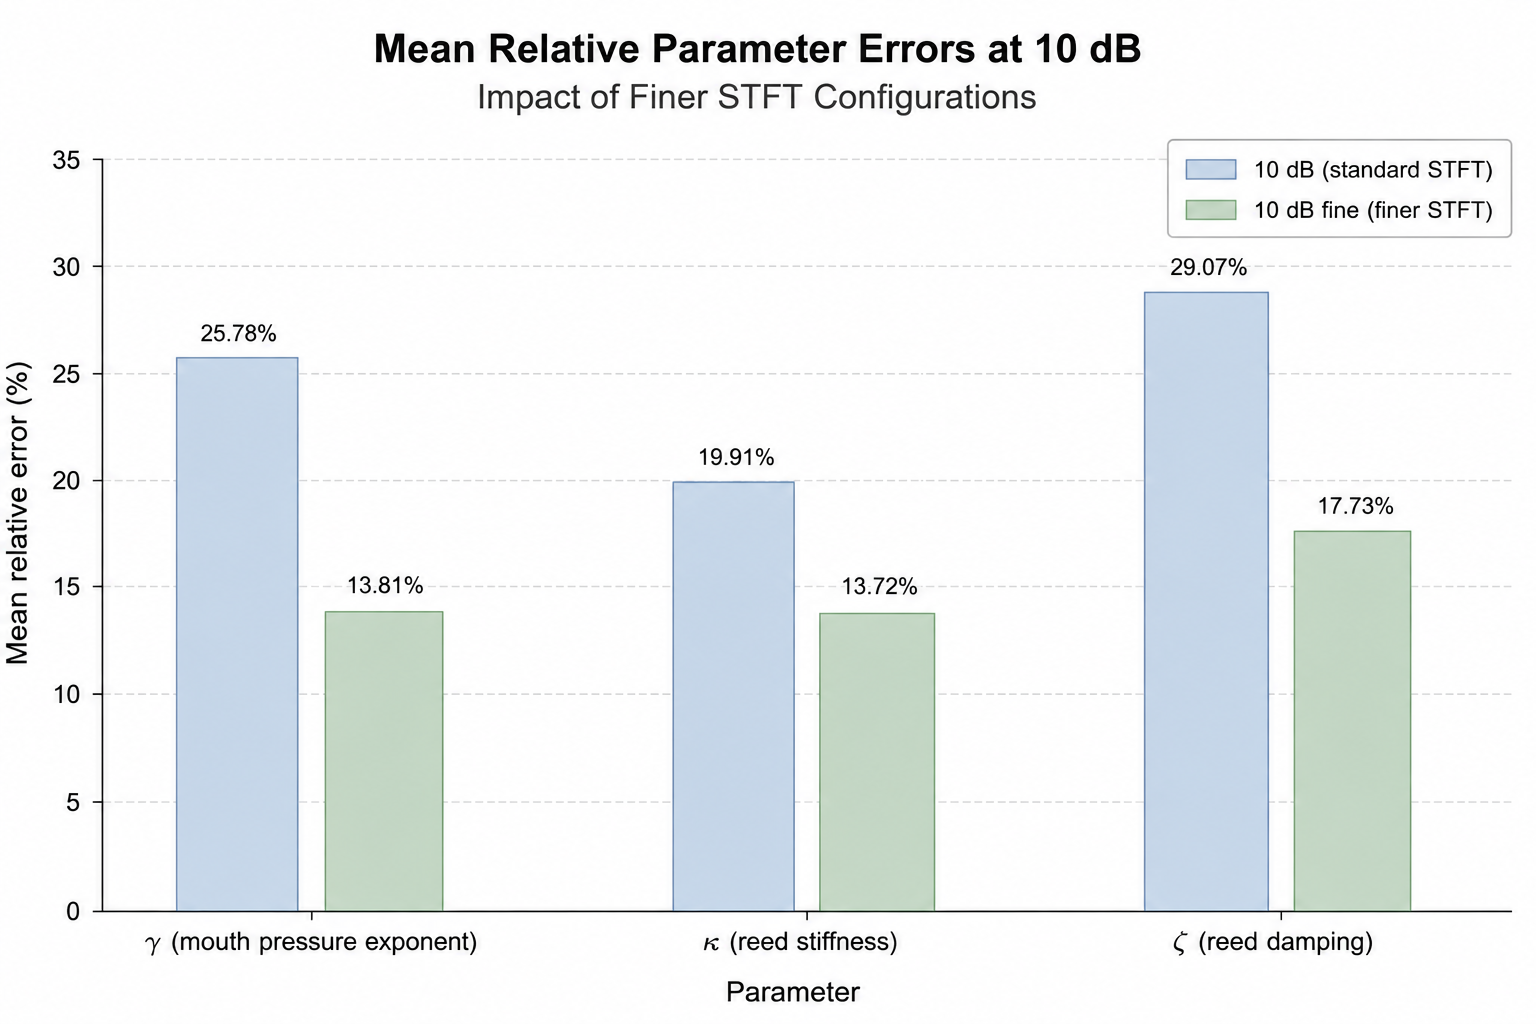
\includegraphics[width=0.9\linewidth,keepaspectratio]{../Images/histo_improv_noisy.png}\hspace{0.0em}%
        \label{fig:improvement_error_noisy}  
    \end{center}

\vspace{-0.2cm}

\orangebox{0.96\linewidth}{
\small
The spectral-loss design significantly improves robustness at low SNR.
}

\end{columns}

\end{frame}

% =============================================================================
% REED-LAW IDENTIFICATION UNDER NOISE
% =============================================================================
\begin{frame}{Reed-Law Identification under Noisy Observations}

\vspace{-0.20cm}

\begin{columns}[T,onlytextwidth]

% -------------------------------------------------------------------------
% LEFT COLUMN : TABLE
% -------------------------------------------------------------------------
\column{0.43\textwidth}

\small

\textbf{Identification accuracy}

\vspace{0.15cm}

\begin{center}

\scriptsize

\begin{tabular}{lccc}
\toprule
Observation
& Rel. error
& Max. error
& $\ell_{\rm NN}(1)$ \\
\midrule

Noise-free
& $0.840\%$
& $2.183\times10^{-2}$
& $0.9963$ \\

$40$ dB
& $0.890\%$
& $2.251\times10^{-2}$
& $0.9956$ \\

$30$ dB
& $0.683\%$
& $1.749\times10^{-2}$
& $0.9970$ \\

$20$ dB
& $0.724\%$
& $1.077\times10^{-2}$
& $1.0060$ \\

$10$ dB
& $13.944\%$
& $2.121\times10^{-1}$
& $1.1407$ \\

\bottomrule
\end{tabular}

\end{center}

\vspace{0.25cm}

\greenbox{0.94\linewidth}{
\small
For moderate noise levels
($20$--$40$ dB),
the relative error remains below $1\%$.
}

\vspace{0.20cm}

\orangebox{0.94\linewidth}{
\small
At $10$ dB, the identification degrades strongly:
the relative error increases to
\[
13.944\%.
\]
}

% -------------------------------------------------------------------------
% RIGHT COLUMN : RECONSTRUCTED FUNCTIONS
% -------------------------------------------------------------------------
\column{0.53\textwidth}

\small

\textbf{Reconstructed reed opening laws}

\vspace{-0.10cm}

\begin{center}

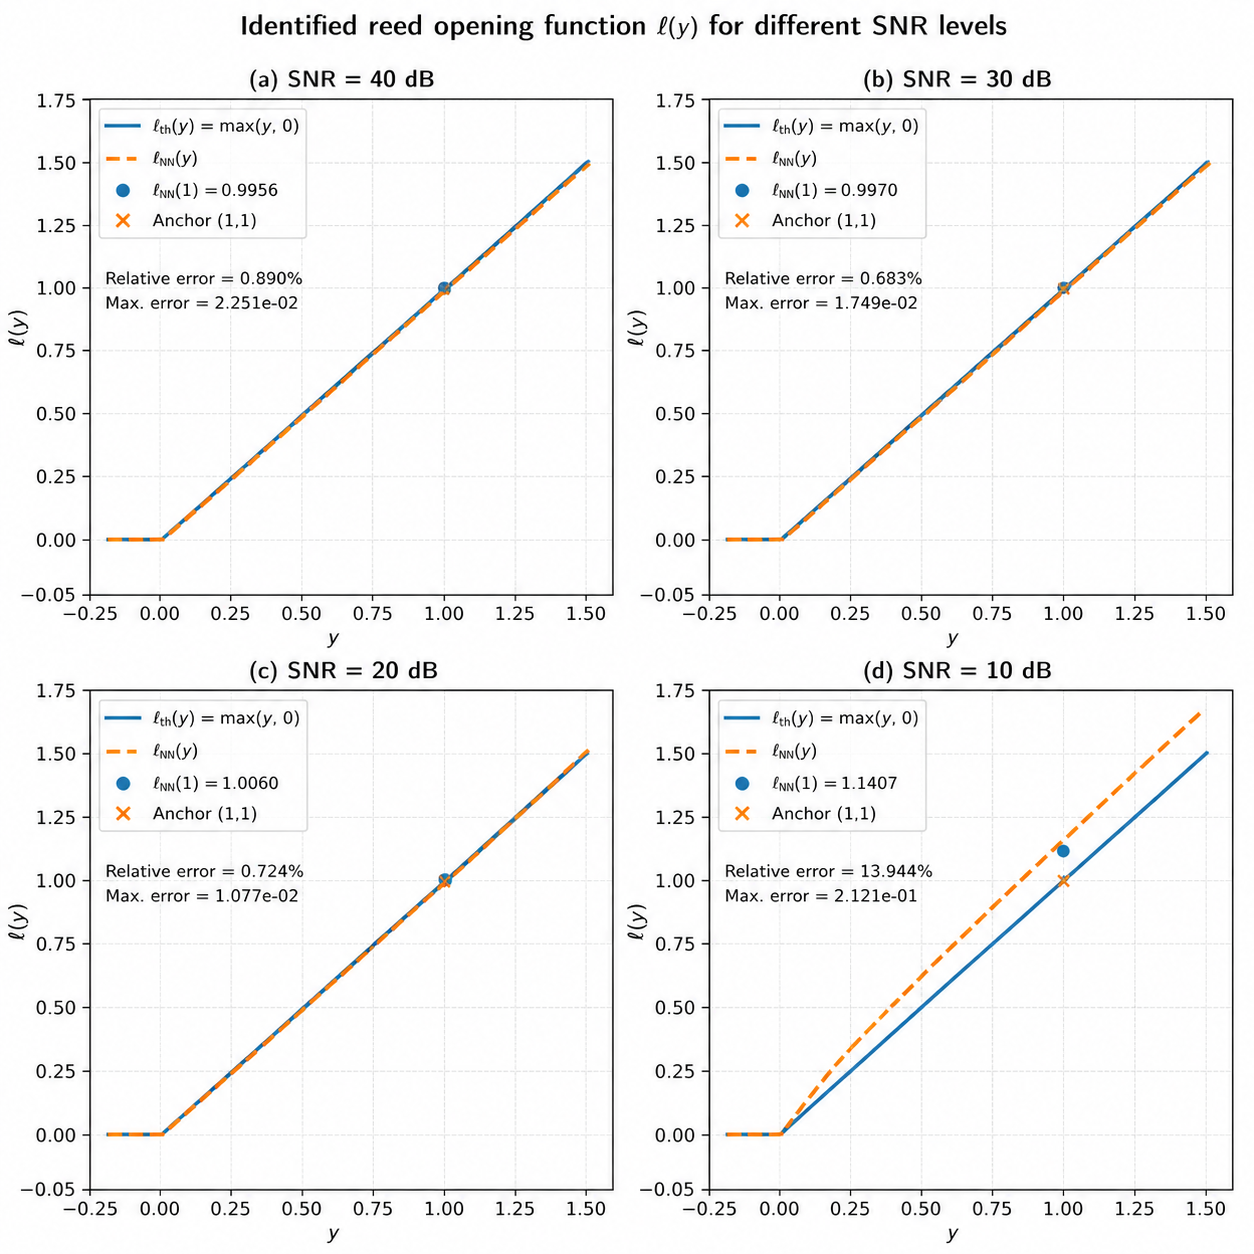
\includegraphics[
    width=0.62\linewidth,
    keepaspectratio
]{../Images/all_ell_y_w_noise.png}

\vspace{-0.05cm}

{\scriptsize
Comparison with the theoretical law
$\ell_{\rm th}(y)=\max(y,0)$
for different SNR levels.
}

\end{center}

\vspace{0.10cm}

\bluebox{0.94\linewidth}{
\small
The identification is relatively insensitive
to moderate noise, but a clear loss of accuracy
appears at $10$ dB.
}

\end{columns}

\end{frame}

% =============================================================================
% CONCLUSION
% =============================================================================
\begin{frame}{Conclusion}

\begin{columns}[T,onlytextwidth]

% -------------------------------------------------------------------------
% LEFT COLUMN
% -------------------------------------------------------------------------
\column{0.50\textwidth}

\textbf{Main contributions}

\vspace{0.18cm}

\begin{itemize}

    \item<1-> \alt<1>{
        \textcolor{mainblue}{
            \textbf{Validated DG solver for the coupled reed model.}
        }
    }{
        \textcolor{gray!55}{
            Validated DG solver for the coupled reed model.
        }
    }

    \item<2-> \alt<2>{
        \textcolor{mainblue}{
            \textbf{End-to-end differentiable implementation in JAX.}
        }
    }{
        \textcolor{gray!55}{
            End-to-end differentiable implementation in JAX.
        }
    }

    \item<3-> \alt<3>{
        \textcolor{mainblue}{
            \textbf{Calibration of $\gamma$, $\kappa$ and $\zeta$.}
        }
    }{
        \textcolor{gray!55}{
            Calibration of $\gamma$, $\kappa$ and $\zeta$.
        }
    }

    \item<4-> \alt<4>{
        \textcolor{mainblue}{
            \textbf{Identification of the reed opening law $\ell(y)$.}
        }
    }{
        \textcolor{gray!55}{
            Identification of the reed opening law $\ell(y)$.
        }
    }

    \item<5-> \alt<5>{
        \textcolor{mainblue}{
            \textbf{Robustness analysis under noisy observations.}
        }
    }{
        \textcolor{gray!55}{
            Robustness analysis under noisy observations.
        }
    }

\end{itemize}


% -------------------------------------------------------------------------
% RIGHT COLUMN
% -------------------------------------------------------------------------
\column{0.46\textwidth}

\small

\textbf{Main findings}

\vspace{0.18cm}

\only<1>{
\greenbox{0.96\linewidth}{
\small
\textbf{Solver validation}\\[0.06cm]
Analytical tests and comparisons with OpenWind
confirm the accuracy of the numerical solver
in both time and frequency domains.
}
}

\only<2>{
\greenbox{0.96\linewidth}{
\small
\textbf{Differentiable implementation}\\[0.06cm]
JAX enables gradients to be propagated
through the complete numerical simulation.
}
}

\only<3>{
\greenbox{0.96\linewidth}{
\small
\textbf{Accurate parameter recovery}\\[0.06cm]
$\gamma$, $\kappa$ and $\zeta$ are accurately recovered
for most noise-free synthetic observations.
}
}

\only<4>{
\bluebox{0.96\linewidth}{
\small
\textbf{Beyond scalar calibration}\\[0.06cm]
The same framework can recover an unknown
constitutive law $\ell(y)$ from acoustic observations.
}
}

\only<5>{
\orangebox{0.96\linewidth}{
\small
\textbf{Robustness to noise}\\[0.06cm]
Noise degrades parameter recovery,
but the choice of the spectral loss can substantially
improve calibration robustness.
}
}

\end{columns}

\vfill

\only<5>{
\centering
{\large\color{mainblue}\bfseries
Differentiable physical modelling provides a viable framework
for inverse calibration in musical acoustics.}
}

\end{frame}

% =============================================================================
% PERSPECTIVES
% =============================================================================
% =============================================================================
% PERSPECTIVES
% =============================================================================
\begin{frame}{Perspectives}

\small

\textbf{From synthetic calibration to real-world applications}

\vspace{0.25cm}

% -------------------------------------------------------------------------
% 1. ROBUSTNESS
% -------------------------------------------------------------------------
\greenbox{0.94\linewidth}{
\begin{minipage}[c]{0.20\linewidth}
\centering
\textbf{\large Robustness}
\end{minipage}
\hfill
\begin{minipage}[c]{0.73\linewidth}
Improve spectral objectives and optimization strategies
to obtain more reliable calibration under noisy observations.
\end{minipage}
}

\vspace{0.18cm}

% -------------------------------------------------------------------------
% 2. IDENTIFIABILITY
% -------------------------------------------------------------------------
\bluebox{0.94\linewidth}{
\begin{minipage}[c]{0.20\linewidth}
\centering
\textbf{\large Identifiability}
\end{minipage}
\hfill
\begin{minipage}[c]{0.73\linewidth}
Investigate weakly observable parameters and exploit
multiple observations to better constrain the inverse problem.
\end{minipage}
}

\vspace{0.18cm}

% -------------------------------------------------------------------------
% 3. MODEL IDENTIFICATION
% -------------------------------------------------------------------------
\purplebox{0.94\linewidth}{
\begin{minipage}[c]{0.20\linewidth}
\centering
\textbf{\large Model}
\end{minipage}
\hfill
\begin{minipage}[c]{0.73\linewidth}
Extend model identification beyond $\ell(y)$,
for example to richer reed laws or a time-dependent excitation $\gamma(t)$.
\end{minipage}
}

\vspace{0.18cm}

% -------------------------------------------------------------------------
% 4. EXPERIMENTAL DATA
% -------------------------------------------------------------------------
\orangebox{0.94\linewidth}{
\begin{minipage}[c]{0.20\linewidth}
\centering
\textbf{\large Experiments}
\end{minipage}
\hfill
\begin{minipage}[c]{0.73\linewidth}
Move towards experimental recordings:
signal scaling and normalization,
geometry uncertainty and model--data mismatch.
\end{minipage}
}

\vspace{0.30cm}

\centering

{\large\color{mainblue}\bfseries
Towards automatic calibration of physical models\\
from real musical instrument recordings.}


\end{frame}

% =============================================================================
% ACKNOWLEDGEMENTS
% =============================================================================
\begin{frame}{Acknowledgements}

\centering

\vspace{0.25cm}

{\large
I would like to thank everyone who contributed to this work.
}

\vspace{0.55cm}

\begin{columns}[T,onlytextwidth]

% -------------------------------------------------------------------------
% LEFT COLUMN
% -------------------------------------------------------------------------
\column{0.47\textwidth}

\bluebox{0.92\linewidth}{
\large
\textbf{Academic supervision}
\\[0.25cm]

\normalsize
Emmanuel Franck
\\[0.12cm]
Laurent Navoret
\\[0.12cm]
Victor Michel-Dansac

\vspace{0.15cm}

\scriptsize
IRMA -- Université de Strasbourg
}

% -------------------------------------------------------------------------
% RIGHT COLUMN
% -------------------------------------------------------------------------
\column{0.47\textwidth}

\purplebox{0.92\linewidth}{
\large
\textbf{Scientific collaboration}
\\[0.25cm]

\normalsize
Juliette Chabassier
\\[0.12cm]
Alexis Thibault

\vspace{0.15cm}

\scriptsize
Modartt
}

\end{columns}

\vspace{0.65cm}

\greenbox{0.78\linewidth}{
\small
Thank you for your guidance, scientific discussions,
feedback and support throughout this project.
}

\vfill

{\Large\color{mainblue}\bfseries
Thank you for your attention}


\end{frame}

\begin{frame}[allowframebreaks]{References}
\printbibliography
\end{frame}

% =============================================================================
% USE OF ARTIFICIAL INTELLIGENCE
% =============================================================================
\begin{frame}{Use of Artificial Intelligence Assistance}

\small
\vspace{-0.1cm}
Some parts of this work were prepared with the assistance of
\textbf{ChatGPT} (OpenAI, GPT-4 / GPT-5 family).

\vspace{-0.1cm}

\begin{columns}[T,onlytextwidth]

% -------------------------------------------------------------------------
% LEFT COLUMN
% -------------------------------------------------------------------------
\column{0.48\textwidth}

\bluebox{0.94\linewidth}{
\textbf{Code development}
\\[0.10cm]
\begin{itemize}
    \item Code support and debugging
    \item Ghost-cell implementation
    \item Argument parsing and automation
    \item Code documentation
\end{itemize}
}

\vspace{0.1cm}

\greenbox{0.94\linewidth}{
\textbf{Scientific methodology}
\\[0.10cm]
\begin{itemize}
    \item Methodological discussions
    \item Performance metrics
    \item Discussion of adjoint methods
    \item Physical modelling examples
\end{itemize}
}


% -------------------------------------------------------------------------
% RIGHT COLUMN
% -------------------------------------------------------------------------
\column{0.48\textwidth}

\purplebox{0.94\linewidth}{
\textbf{Scientific writing}
\\[0.10cm]
\begin{itemize}
    \item Reformulation and organization
    \item Bibliography assistance
    \item Literature searches
    \item Report structure
\end{itemize}
}

\vspace{0.1cm}

\orangebox{0.94\linewidth}{
\textbf{Figures \& presentation}
\\[0.10cm]
\begin{itemize}
    \item Figure and diagram design
    \item Layout improvements
    \item \LaTeX{} assistance
    \item Presentation of results
\end{itemize}
}

\end{columns}

\vspace{0.1cm}

\centering

\bluebox{0.88\linewidth}{
\small
\textbf{All AI-generated outputs were systematically verified,
adapted and corrected.}\\[0.05cm]
Full responsibility for the scientific content and integrity
of this work remains with the author.
}

\end{frame}
% =============================================================================
% 4. NUMERICAL SOLVER
% =============================================================================
\begin{frame}{Numerical Solver}
\vspace{-0.15cm}

\begin{columns}[T,onlytextwidth]

% =====================================================================
% LEFT COLUMN
% =====================================================================
\column{0.46\textwidth}

\small
\textbf{Numerical ingredients}

\vspace{0.2cm}

\begin{itemize}

    % -----------------------------------------------------------------
    % 1. CONSERVATIVE FORMULATION
    % -----------------------------------------------------------------
    \item<1-> \alt<1>{
        \textcolor{mainblue}{
            \textbf{Conservative formulation of the acoustic system.}
        }
    }{
        \textcolor{gray!55}{
            Conservative formulation of the acoustic system.
        }
    }

    % -----------------------------------------------------------------
    % 2. DG + RUSANOV
    % -----------------------------------------------------------------
    \item<1-> \alt<2>{
        \textcolor{mainblue}{
            \textbf{Discontinuous Galerkin discretization and Rusanov flux.}
            \textsuperscript{1}
        }
    }{
        \textcolor{gray!55}{
            Discontinuous Galerkin discretization and Rusanov flux.
        }
    }

    % -----------------------------------------------------------------
    % 3. CHARACTERISTIC VARIABLES
    % -----------------------------------------------------------------
    \item<1-> \alt<3>{
        \textcolor{mainblue}{
            \textbf{Characteristic variables and boundary conditions.}
        }
    }{
        \textcolor{gray!55}{
            Characteristic variables and boundary conditions.
        }
    }

    % -----------------------------------------------------------------
    % 4. TIME INTEGRATION
    % -----------------------------------------------------------------
    \item<1-> \alt<4>{
        \textcolor{mainblue}{
            \textbf{RK2 time integration of the coupled system.}
        }
    }{
        \textcolor{gray!55}{
            RK2 time integration of the coupled system.
        }
    }

    % -----------------------------------------------------------------
    % 5. NONLINEAR COUPLING
    % -----------------------------------------------------------------
    \item<1-> \alt<5>{
        \textcolor{mainblue}{
            \textbf{Damped Newton method for nonlinear coupling.}
        }
    }{
        \textcolor{gray!55}{
            Damped Newton method for nonlinear coupling.
        }
    }

\end{itemize}

\vspace{0.15cm}

\greenbox{0.94\linewidth}{
Implementation in \textbf{JAX}: the complete solver can be differentiated.
}

% Reference displayed only during the DG overlay
\only<2>{
    \vspace{0.15cm}

    {\scriptsize
\textsuperscript{1}
\cite{HesthavenWarburton2008}
Hesthaven and Warburton (2008),
\emph{Nodal Discontinuous Galerkin Methods}.
}

}


% =====================================================================
% RIGHT COLUMN
% =====================================================================
\column{0.50\textwidth}


% ---------------------------------------------------------------------
% STEP 1 : CONSERVATIVE FORMULATION
% ---------------------------------------------------------------------
\only<1>{

\textbf{\color{mainblue}Conservative formulation}

\vspace{0.1cm}

Starting from the acoustic equations,

\vspace{-0.2cm}

\[
\frac{S(x)}{cS^*}\partial_t p+\partial_x v=0,
\qquad
\frac{S^*}{cS(x)}\partial_t v+\partial_x p=0,
\]

\vspace{-0.2cm}

we introduce the conservative variables

\vspace{-0.05cm}

\[
\widetilde{\mathbf u}
=
(\widetilde p,\widetilde v)^T,
\qquad
\widetilde p
=
\frac{S(x)}{cS^*}p,
\qquad
\widetilde v
=
\frac{S^*}{cS(x)}v.
\]

\vspace{-0.2cm}

The system becomes

\[
\partial_t \widetilde{\mathbf u}
+
\partial_x
\left(
A(x)\widetilde{\mathbf u}
\right)
=
0,
\]

where

\vspace{-0.2cm}

\scriptsize
\[
A(x)
=
\begin{pmatrix}
0 &
\dfrac{cS(x)}{S^\ast}
\\[0.4em]
\dfrac{cS^\ast}{S(x)}
&
0
\end{pmatrix}.
\]

\vspace{0.05cm}

\bluebox{0.94\linewidth}{
\small
Hyperbolic conservative system adapted to DG discretization.
}

}


% ---------------------------------------------------------------------
% STEP 2 : DG + RUSANOV
% ---------------------------------------------------------------------
\only<2>{

\textbf{\color{mainblue}DG spatial discretization}

\vspace{0.1cm}

With
\[
\mathbf F(x,\widetilde{\mathbf u})
=
A(x)\widetilde{\mathbf u},
\]
on each element $K_j$,

\vspace{-0.2cm}

\[
\int_{K_j}
\partial_t \widetilde{\mathbf u}_h
\,\boldsymbol\varphi\,dx
-
\int_{K_j}
\mathbf F(\widetilde{\mathbf u}_h)
\,\partial_x\boldsymbol\varphi\,dx
+
\widehat{\mathbf F}\,
\boldsymbol\varphi
\Big|_{\partial K_j}
=
0.
\]

\vspace{0.05cm}

At element interfaces, the Rusanov flux is

\vspace{-0.15cm}

\[
\boxed{
\widehat{\mathbf F}
=
\frac{1}{2}
\left[
\mathbf F(\mathbf u^-)
+
\mathbf F(\mathbf u^+)
\right]
-
\frac{c}{2}
\left(
\mathbf u^+
-
\mathbf u^-
\right)
}
\]

\vspace{0.15cm}

\bluebox{0.94\linewidth}{
\small
The numerical flux couples neighbouring DG elements.
}

}


% ---------------------------------------------------------------------
% STEP 3 : CHARACTERISTIC VARIABLES
% ---------------------------------------------------------------------
\only<3>{

\textbf{\color{mainblue}Characteristic variables at the boundaries}

\vspace{0.1cm}

The two characteristic speeds are

\vspace{-0.2cm}

\[
\boxed{\lambda_-=-c},
\qquad
\boxed{\lambda_+=+c}.
\]

The associated characteristic variables are

\vspace{-0.2cm}

\[
\boxed{
w^\pm
=
\widetilde v
\pm
\frac{S^\ast}{S(x)}
\widetilde p
}
\]

\vspace{-0.55cm}

\begin{center}
    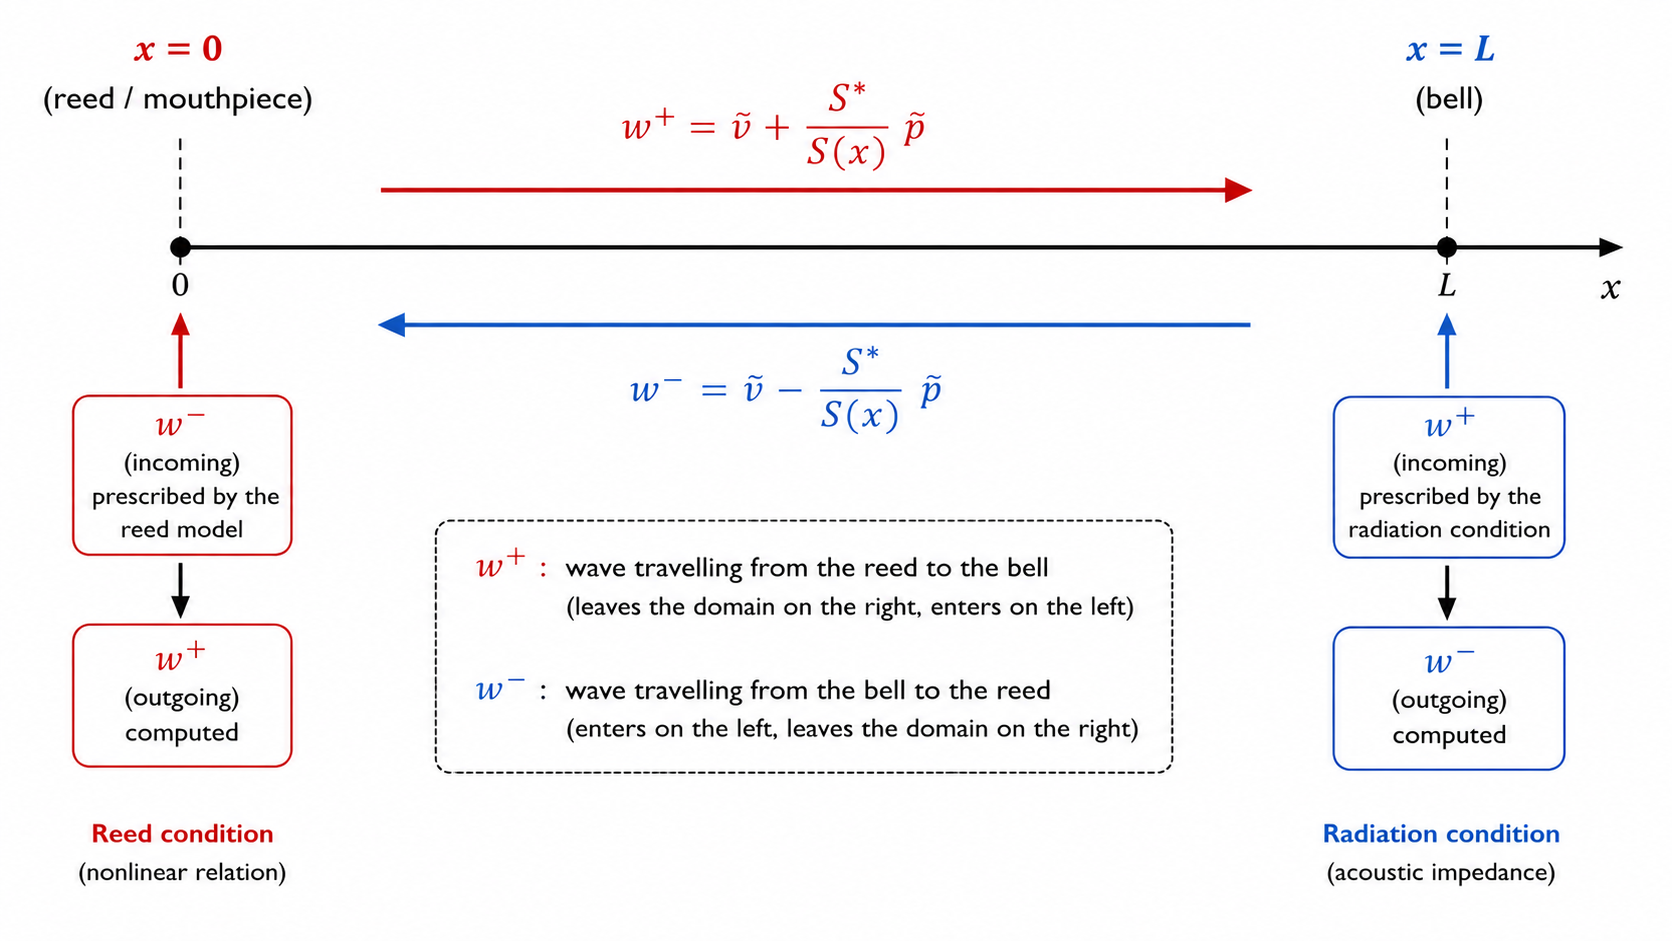
\includegraphics[
        width=0.8\linewidth,
        keepaspectratio
    ]{../Images/characteristics_propagation.png}

    \par
    \scriptsize
    Schematic representation of the local characteristic
    directions of the acoustic system.
\end{center}

}


% ---------------------------------------------------------------------
% STEP 4 : TIME INTEGRATION
% ---------------------------------------------------------------------
\only<4>{

\textbf{\color{mainblue}Time integration}

\vspace{0.1cm}

After spatial discretization, the coupled system is written as

\vspace{-0.35cm}

\[
\frac{d\mathbf U}{dt}
=
\mathcal R(\mathbf U),
\]

where $\mathbf U$ contains the acoustic,
radiative and reed variables.

\vspace{0.15cm}

A second-order explicit Runge--Kutta scheme is used:

\vspace{-0.45cm}

\[
\mathbf U^{n+\frac12}
=
\mathbf U^n
+
\frac{\Delta t}{2}\,
\mathcal R(\mathbf U^n),
\]
\vspace{-0.25cm}
\[
\boxed{
\mathbf U^{n+1}
=
\mathbf U^n
+
\Delta t\,
\mathcal R\!\left(\mathbf U^{n+\frac12}\right)
}
\]


\bluebox{0.94\linewidth}{
\small
The acoustic field, radiation variable and reed dynamics
are advanced with the same explicit RK2 scheme.
}

}


% ---------------------------------------------------------------------
% STEP 5 : NONLINEAR REED COUPLING — DEFINITION OF G
% ---------------------------------------------------------------------
\only<5>{

\textbf{\color{mainblue}Nonlinear reed coupling}

\vspace{0.10cm}

At the mouthpiece, the outgoing characteristic

\vspace{-0.3cm}

\[
w^-
=
\widetilde v_L
-
k_{\rm char}\widetilde p_L,
\qquad
k_{\rm char}
=
\frac{S^\ast}{S_L},
\]

\vspace{-0.3cm}

is known from the interior DG solution.

The incoming characteristic $w^+$ determines

\vspace{-0.5cm}

\[
p
=
\frac{c}{2}(w^+-w^-),
\qquad
v
=
\frac{c}{2k_{\rm char}}(w^++w^-).
\]

\vspace{-0.2cm}

Substitution into the nonlinear reed condition gives

\vspace{-0.6cm}

\[
\boxed{
\begin{aligned}
G(w^+)
={}&
-\frac{c}{2k_{\rm char}}
(w^++w^-)
\\
&+
\zeta\ell(y)
F\!\left(
\gamma
-
\frac{c}{2}(w^+-w^-)
\right)
+
\varepsilon
\frac{\kappa}{\omega_r}
\dot y .
\end{aligned}
}
\]

\vspace{-0.25cm}

\bluebox{0.94\linewidth}{
\small
The nonlinear boundary condition is reduced to
a scalar equation for the incoming characteristic $w^+$.
}

}

\end{columns}

\end{frame}

% =============================================================================
% NUMERICAL SOLVER — NONLINEAR SOLVE
% =============================================================================
\begin{frame}{Numerical Solver}
\vspace{-0.15cm}

\begin{columns}[T,onlytextwidth]

% =====================================================================
% LEFT COLUMN
% =====================================================================
\column{0.46\textwidth}

\small
\textbf{Numerical ingredients}

\vspace{0.2cm}

\begin{itemize}

    \item \textcolor{gray!55}{
        Conservative formulation of the acoustic system.
    }

    \item \textcolor{gray!55}{
        Discontinuous Galerkin discretization and Rusanov flux.
    }

    \item \textcolor{gray!55}{
        Characteristic variables and boundary conditions.
    }

    \item \textcolor{gray!55}{
        RK2 time integration of the coupled system.
    }

    \item \textcolor{mainblue}{
        \textbf{Damped Newton method for nonlinear coupling.}
    }

\end{itemize}

\vspace{0.15cm}

\greenbox{0.94\linewidth}{
Implementation in \textbf{JAX}: the complete solver can be differentiated.
}


% =====================================================================
% RIGHT COLUMN
% =====================================================================
\column{0.50\textwidth}

\textbf{\color{mainblue}Damped Newton solver}

\vspace{0.10cm}

The incoming characteristic is determined by
\vspace{-0.3cm}
\[
\boxed{
G(w^+)=0
}
\]

\vspace{-0.1cm}

and solved iteratively using
\vspace{-0.3cm}
\[
\boxed{
w^{+,(k+1)}
=
w^{+,(k)}
-
\lambda
\frac{G(w^{+,(k)})}
     {G'(w^{+,(k)})}
}
\]

with $0<\lambda\leq1$ the damping parameter.

\vspace{0.10cm}

Once $w^+$ is obtained, the boundary state is reconstructed:
\vspace{-0.2cm}
\[
\widetilde v_{\rm ext}
=
\frac{w^++w^-}{2},
\qquad
\widetilde p_{\rm ext}
=
\frac{w^+-w^-}{2k_{\rm char}}.
\]

\vspace{-0.3cm}

\bluebox{0.94\linewidth}{
\small
The reed condition determines the incoming characteristic
from the outgoing characteristic provided by the DG solution.
}

\end{columns}

\end{frame}

\begin{frame}{Appendix -- DG Approximation Space}

Let
\[
\mathcal T_h=\{K_j\}_{j=1}^{N}
\]
be a partition of the acoustic domain $(0,L)$.

\vspace{0.2cm}

The discontinuous piecewise-linear approximation space is

\[
\boxed{
V_h^1
=
\left\{
q_h\in L^2(0,L)
\;:\;
q_h|_{K_j}\in\mathbb P_1(K_j),
\quad
\forall K_j\in\mathcal T_h
\right\}.
}
\]

The acoustic state is approximated by

\[
\boxed{
\widetilde{\mathbf u}_h
=
(\widetilde p_h,\widetilde v_h)^T
\in (V_h^1)^2.
}
\]

For each interface $x_{j+\frac12}$, the discontinuity of the
approximation leads to two traces,

\[
\widetilde{\mathbf u}_h^-
=
\lim_{x\to x_{j+\frac12}^{-}}
\widetilde{\mathbf u}_h(x),
\qquad
\widetilde{\mathbf u}_h^+
=
\lim_{x\to x_{j+\frac12}^{+}}
\widetilde{\mathbf u}_h(x),
\]

which are coupled through the numerical flux.

\end{frame}



\end{document}
